\documentclass{article}
\usepackage[final]{neurips_2025}  % NEURIPS style (neurips_2025.sty is in paper_draft/)
% [final] alone leaves the footer's track name undefined; keep it blank (this paper is not a conference publication)
\makeatletter\providecommand{\@trackname}{}\makeatother
\usepackage[hidelinks]{hyperref}  % REQUIRED: clickable links
\usepackage{booktabs}  % REQUIRED: professional tables
\usepackage{graphicx}
\usepackage{amsmath,amssymb}
\usepackage[T1]{fontenc}
\usepackage{enumitem}
\usepackage{multirow}
\usepackage{tikz}
\usetikzlibrary{positioning,arrows.meta}
\usepackage{algorithm}
\usepackage[noend]{algpseudocode}

% Import command files
%%%%% MATH NOTATION MACROS %%%%%
% Standard math notation for academic papers
% Import with: %%%%% MATH NOTATION MACROS %%%%%
% Standard math notation for academic papers
% Import with: %%%%% MATH NOTATION MACROS %%%%%
% Standard math notation for academic papers
% Import with: \input{commands/math}

\usepackage{amsmath,amsfonts,bm}

%%%%%%%%%%%%%%%%%%%%%%%%%%%%%%%%%%%%%%%%%%%%%%%%%%%%%%%%%%%%%%%%%
% FIGURE AND SECTION REFERENCES
%%%%%%%%%%%%%%%%%%%%%%%%%%%%%%%%%%%%%%%%%%%%%%%%%%%%%%%%%%%%%%%%%

% Mark sections of captions for referring to divisions of figures
\newcommand{\figleft}{{\em (Left)}}
\newcommand{\figcenter}{{\em (Center)}}
\newcommand{\figright}{{\em (Right)}}
\newcommand{\figtop}{{\em (Top)}}
\newcommand{\figbottom}{{\em (Bottom)}}
\newcommand{\captiona}{{\em (a)}}
\newcommand{\captionb}{{\em (b)}}
\newcommand{\captionc}{{\em (c)}}
\newcommand{\captiond}{{\em (d)}}

% Figure references
\def\figref#1{figure~\ref{#1}}
\def\Figref#1{Figure~\ref{#1}}
\def\twofigref#1#2{figures \ref{#1} and \ref{#2}}
\def\quadfigref#1#2#3#4{figures \ref{#1}, \ref{#2}, \ref{#3} and \ref{#4}}

% Section references
\def\secref#1{section~\ref{#1}}
\def\Secref#1{Section~\ref{#1}}
\def\twosecrefs#1#2{sections \ref{#1} and \ref{#2}}
\def\secrefs#1#2#3{sections \ref{#1}, \ref{#2} and \ref{#3}}

% Equation references
\def\eqref#1{equation~\ref{#1}}
\def\Eqref#1{Equation~\ref{#1}}
\def\plaineqref#1{\ref{#1}}

% Algorithm references
\def\algref#1{algorithm~\ref{#1}}
\def\Algref#1{Algorithm~\ref{#1}}
\def\twoalgref#1#2{algorithms \ref{#1} and \ref{#2}}
\def\Twoalgref#1#2{Algorithms \ref{#1} and \ref{#2}}

% Table references
\def\tabref#1{table~\ref{#1}}
\def\Tabref#1{Table~\ref{#1}}

% Chapter references
\def\chapref#1{chapter~\ref{#1}}
\def\Chapref#1{Chapter~\ref{#1}}

%%%%%%%%%%%%%%%%%%%%%%%%%%%%%%%%%%%%%%%%%%%%%%%%%%%%%%%%%%%%%%%%%
% BASIC MATH DEFINITIONS
%%%%%%%%%%%%%%%%%%%%%%%%%%%%%%%%%%%%%%%%%%%%%%%%%%%%%%%%%%%%%%%%%

\def\ceil#1{\lceil #1 \rceil}
\def\floor#1{\lfloor #1 \rfloor}
\def\1{\bm{1}}
\def\eps{{\epsilon}}

% Common operators
\DeclareMathOperator*{\argmax}{arg\,max}
\DeclareMathOperator*{\argmin}{arg\,min}
\DeclareMathOperator{\sign}{sign}
\DeclareMathOperator{\Tr}{Tr}
\let\ab\allowbreak

%%%%%%%%%%%%%%%%%%%%%%%%%%%%%%%%%%%%%%%%%%%%%%%%%%%%%%%%%%%%%%%%%
% VECTORS (lowercase bold)
%%%%%%%%%%%%%%%%%%%%%%%%%%%%%%%%%%%%%%%%%%%%%%%%%%%%%%%%%%%%%%%%%

\def\vzero{{\bm{0}}}
\def\vone{{\bm{1}}}
\def\vmu{{\bm{\mu}}}
\def\vtheta{{\bm{\theta}}}
\def\va{{\bm{a}}}
\def\vb{{\bm{b}}}
\def\vc{{\bm{c}}}
\def\vd{{\bm{d}}}
\def\ve{{\bm{e}}}
\def\vf{{\bm{f}}}
\def\vg{{\bm{g}}}
\def\vh{{\bm{h}}}
\def\vi{{\bm{i}}}
\def\vj{{\bm{j}}}
\def\vk{{\bm{k}}}
\def\vl{{\bm{l}}}
\def\vm{{\bm{m}}}
\def\vn{{\bm{n}}}
\def\vo{{\bm{o}}}
\def\vp{{\bm{p}}}
\def\vq{{\bm{q}}}
\def\vr{{\bm{r}}}
\def\vs{{\bm{s}}}
\def\vt{{\bm{t}}}
\def\vu{{\bm{u}}}
\def\vv{{\bm{v}}}
\def\vw{{\bm{w}}}
\def\vx{{\bm{x}}}
\def\vy{{\bm{y}}}
\def\vz{{\bm{z}}}

%%%%%%%%%%%%%%%%%%%%%%%%%%%%%%%%%%%%%%%%%%%%%%%%%%%%%%%%%%%%%%%%%
% MATRICES (uppercase bold)
%%%%%%%%%%%%%%%%%%%%%%%%%%%%%%%%%%%%%%%%%%%%%%%%%%%%%%%%%%%%%%%%%

\def\mA{{\bm{A}}}
\def\mB{{\bm{B}}}
\def\mC{{\bm{C}}}
\def\mD{{\bm{D}}}
\def\mE{{\bm{E}}}
\def\mF{{\bm{F}}}
\def\mG{{\bm{G}}}
\def\mH{{\bm{H}}}
\def\mI{{\bm{I}}}
\def\mJ{{\bm{J}}}
\def\mK{{\bm{K}}}
\def\mL{{\bm{L}}}
\def\mM{{\bm{M}}}
\def\mN{{\bm{N}}}
\def\mO{{\bm{O}}}
\def\mP{{\bm{P}}}
\def\mQ{{\bm{Q}}}
\def\mR{{\bm{R}}}
\def\mS{{\bm{S}}}
\def\mT{{\bm{T}}}
\def\mU{{\bm{U}}}
\def\mV{{\bm{V}}}
\def\mW{{\bm{W}}}
\def\mX{{\bm{X}}}
\def\mY{{\bm{Y}}}
\def\mZ{{\bm{Z}}}
\def\mBeta{{\bm{\beta}}}
\def\mPhi{{\bm{\Phi}}}
\def\mLambda{{\bm{\Lambda}}}
\def\mSigma{{\bm{\Sigma}}}

%%%%%%%%%%%%%%%%%%%%%%%%%%%%%%%%%%%%%%%%%%%%%%%%%%%%%%%%%%%%%%%%%
% CALLIGRAPHIC (mathcal)
%%%%%%%%%%%%%%%%%%%%%%%%%%%%%%%%%%%%%%%%%%%%%%%%%%%%%%%%%%%%%%%%%

\def\gA{{\mathcal{A}}}
\def\gB{{\mathcal{B}}}
\def\gC{{\mathcal{C}}}
\def\gD{{\mathcal{D}}}
\def\gE{{\mathcal{E}}}
\def\gF{{\mathcal{F}}}
\def\gG{{\mathcal{G}}}
\def\gH{{\mathcal{H}}}
\def\gI{{\mathcal{I}}}
\def\gJ{{\mathcal{J}}}
\def\gK{{\mathcal{K}}}
\def\gL{{\mathcal{L}}}
\def\gM{{\mathcal{M}}}
\def\gN{{\mathcal{N}}}
\def\gO{{\mathcal{O}}}
\def\gP{{\mathcal{P}}}
\def\gQ{{\mathcal{Q}}}
\def\gR{{\mathcal{R}}}
\def\gS{{\mathcal{S}}}
\def\gT{{\mathcal{T}}}
\def\gU{{\mathcal{U}}}
\def\gV{{\mathcal{V}}}
\def\gW{{\mathcal{W}}}
\def\gX{{\mathcal{X}}}
\def\gY{{\mathcal{Y}}}
\def\gZ{{\mathcal{Z}}}

%%%%%%%%%%%%%%%%%%%%%%%%%%%%%%%%%%%%%%%%%%%%%%%%%%%%%%%%%%%%%%%%%
% SETS (blackboard bold)
%%%%%%%%%%%%%%%%%%%%%%%%%%%%%%%%%%%%%%%%%%%%%%%%%%%%%%%%%%%%%%%%%

\def\sA{{\mathbb{A}}}
\def\sB{{\mathbb{B}}}
\def\sC{{\mathbb{C}}}
\def\sD{{\mathbb{D}}}
\def\sF{{\mathbb{F}}}
\def\sG{{\mathbb{G}}}
\def\sH{{\mathbb{H}}}
\def\sI{{\mathbb{I}}}
\def\sJ{{\mathbb{J}}}
\def\sK{{\mathbb{K}}}
\def\sL{{\mathbb{L}}}
\def\sM{{\mathbb{M}}}
\def\sN{{\mathbb{N}}}
\def\sO{{\mathbb{O}}}
\def\sP{{\mathbb{P}}}
\def\sQ{{\mathbb{Q}}}
\def\sR{{\mathbb{R}}}
\def\sS{{\mathbb{S}}}
\def\sT{{\mathbb{T}}}
\def\sU{{\mathbb{U}}}
\def\sV{{\mathbb{V}}}
\def\sW{{\mathbb{W}}}
\def\sX{{\mathbb{X}}}
\def\sY{{\mathbb{Y}}}
\def\sZ{{\mathbb{Z}}}

%%%%%%%%%%%%%%%%%%%%%%%%%%%%%%%%%%%%%%%%%%%%%%%%%%%%%%%%%%%%%%%%%
% COMMON MATH SHORTCUTS
%%%%%%%%%%%%%%%%%%%%%%%%%%%%%%%%%%%%%%%%%%%%%%%%%%%%%%%%%%%%%%%%%

% Expectation and variance
\newcommand{\E}{\mathbb{E}}
\newcommand{\Var}{\mathrm{Var}}
\newcommand{\Cov}{\mathrm{Cov}}
\newcommand{\R}{\mathbb{R}}

% Datasets
\newcommand{\train}{\mathcal{D}}
\newcommand{\valid}{\mathcal{D_{\mathrm{valid}}}}
\newcommand{\test}{\mathcal{D_{\mathrm{test}}}}

% Distributions
\newcommand{\laplace}{\mathrm{Laplace}}
\newcommand{\Uniform}{\mathrm{Unif}}
\newcommand{\Normal}{\mathrm{Normal}}
\newcommand{\Categorical}{\mathrm{Categorical}}

% Common functions
\newcommand{\softmax}{\mathrm{softmax}}
\newcommand{\sigmoid}{\sigma}
\newcommand{\KL}{D_{\mathrm{KL}}}

% Norms
\newcommand{\normlzero}{L^0}
\newcommand{\normlone}{L^1}
\newcommand{\normltwo}{L^2}
\newcommand{\normlp}{L^p}
\newcommand{\normmax}{L^\infty}

%%%%%%%%%%%%%%%%%%%%%%%%%%%%%%%%%%%%%%%%%%%%%%%%%%%%%%%%%%%%%%%%%
% DEFINITIONS AND HIGHLIGHTING
%%%%%%%%%%%%%%%%%%%%%%%%%%%%%%%%%%%%%%%%%%%%%%%%%%%%%%%%%%%%%%%%%

% Highlight a newly defined term
\newcommand{\newterm}[1]{{\bf #1}}
\newcommand{\defn}[1]{\textbf{#1}}
\newcommand{\defeq}{\mathrel{\stackrel{\textnormal{\tiny def}}{=}}}


\usepackage{amsmath,amsfonts,bm}

%%%%%%%%%%%%%%%%%%%%%%%%%%%%%%%%%%%%%%%%%%%%%%%%%%%%%%%%%%%%%%%%%
% FIGURE AND SECTION REFERENCES
%%%%%%%%%%%%%%%%%%%%%%%%%%%%%%%%%%%%%%%%%%%%%%%%%%%%%%%%%%%%%%%%%

% Mark sections of captions for referring to divisions of figures
\newcommand{\figleft}{{\em (Left)}}
\newcommand{\figcenter}{{\em (Center)}}
\newcommand{\figright}{{\em (Right)}}
\newcommand{\figtop}{{\em (Top)}}
\newcommand{\figbottom}{{\em (Bottom)}}
\newcommand{\captiona}{{\em (a)}}
\newcommand{\captionb}{{\em (b)}}
\newcommand{\captionc}{{\em (c)}}
\newcommand{\captiond}{{\em (d)}}

% Figure references
\def\figref#1{figure~\ref{#1}}
\def\Figref#1{Figure~\ref{#1}}
\def\twofigref#1#2{figures \ref{#1} and \ref{#2}}
\def\quadfigref#1#2#3#4{figures \ref{#1}, \ref{#2}, \ref{#3} and \ref{#4}}

% Section references
\def\secref#1{section~\ref{#1}}
\def\Secref#1{Section~\ref{#1}}
\def\twosecrefs#1#2{sections \ref{#1} and \ref{#2}}
\def\secrefs#1#2#3{sections \ref{#1}, \ref{#2} and \ref{#3}}

% Equation references
\def\eqref#1{equation~\ref{#1}}
\def\Eqref#1{Equation~\ref{#1}}
\def\plaineqref#1{\ref{#1}}

% Algorithm references
\def\algref#1{algorithm~\ref{#1}}
\def\Algref#1{Algorithm~\ref{#1}}
\def\twoalgref#1#2{algorithms \ref{#1} and \ref{#2}}
\def\Twoalgref#1#2{Algorithms \ref{#1} and \ref{#2}}

% Table references
\def\tabref#1{table~\ref{#1}}
\def\Tabref#1{Table~\ref{#1}}

% Chapter references
\def\chapref#1{chapter~\ref{#1}}
\def\Chapref#1{Chapter~\ref{#1}}

%%%%%%%%%%%%%%%%%%%%%%%%%%%%%%%%%%%%%%%%%%%%%%%%%%%%%%%%%%%%%%%%%
% BASIC MATH DEFINITIONS
%%%%%%%%%%%%%%%%%%%%%%%%%%%%%%%%%%%%%%%%%%%%%%%%%%%%%%%%%%%%%%%%%

\def\ceil#1{\lceil #1 \rceil}
\def\floor#1{\lfloor #1 \rfloor}
\def\1{\bm{1}}
\def\eps{{\epsilon}}

% Common operators
\DeclareMathOperator*{\argmax}{arg\,max}
\DeclareMathOperator*{\argmin}{arg\,min}
\DeclareMathOperator{\sign}{sign}
\DeclareMathOperator{\Tr}{Tr}
\let\ab\allowbreak

%%%%%%%%%%%%%%%%%%%%%%%%%%%%%%%%%%%%%%%%%%%%%%%%%%%%%%%%%%%%%%%%%
% VECTORS (lowercase bold)
%%%%%%%%%%%%%%%%%%%%%%%%%%%%%%%%%%%%%%%%%%%%%%%%%%%%%%%%%%%%%%%%%

\def\vzero{{\bm{0}}}
\def\vone{{\bm{1}}}
\def\vmu{{\bm{\mu}}}
\def\vtheta{{\bm{\theta}}}
\def\va{{\bm{a}}}
\def\vb{{\bm{b}}}
\def\vc{{\bm{c}}}
\def\vd{{\bm{d}}}
\def\ve{{\bm{e}}}
\def\vf{{\bm{f}}}
\def\vg{{\bm{g}}}
\def\vh{{\bm{h}}}
\def\vi{{\bm{i}}}
\def\vj{{\bm{j}}}
\def\vk{{\bm{k}}}
\def\vl{{\bm{l}}}
\def\vm{{\bm{m}}}
\def\vn{{\bm{n}}}
\def\vo{{\bm{o}}}
\def\vp{{\bm{p}}}
\def\vq{{\bm{q}}}
\def\vr{{\bm{r}}}
\def\vs{{\bm{s}}}
\def\vt{{\bm{t}}}
\def\vu{{\bm{u}}}
\def\vv{{\bm{v}}}
\def\vw{{\bm{w}}}
\def\vx{{\bm{x}}}
\def\vy{{\bm{y}}}
\def\vz{{\bm{z}}}

%%%%%%%%%%%%%%%%%%%%%%%%%%%%%%%%%%%%%%%%%%%%%%%%%%%%%%%%%%%%%%%%%
% MATRICES (uppercase bold)
%%%%%%%%%%%%%%%%%%%%%%%%%%%%%%%%%%%%%%%%%%%%%%%%%%%%%%%%%%%%%%%%%

\def\mA{{\bm{A}}}
\def\mB{{\bm{B}}}
\def\mC{{\bm{C}}}
\def\mD{{\bm{D}}}
\def\mE{{\bm{E}}}
\def\mF{{\bm{F}}}
\def\mG{{\bm{G}}}
\def\mH{{\bm{H}}}
\def\mI{{\bm{I}}}
\def\mJ{{\bm{J}}}
\def\mK{{\bm{K}}}
\def\mL{{\bm{L}}}
\def\mM{{\bm{M}}}
\def\mN{{\bm{N}}}
\def\mO{{\bm{O}}}
\def\mP{{\bm{P}}}
\def\mQ{{\bm{Q}}}
\def\mR{{\bm{R}}}
\def\mS{{\bm{S}}}
\def\mT{{\bm{T}}}
\def\mU{{\bm{U}}}
\def\mV{{\bm{V}}}
\def\mW{{\bm{W}}}
\def\mX{{\bm{X}}}
\def\mY{{\bm{Y}}}
\def\mZ{{\bm{Z}}}
\def\mBeta{{\bm{\beta}}}
\def\mPhi{{\bm{\Phi}}}
\def\mLambda{{\bm{\Lambda}}}
\def\mSigma{{\bm{\Sigma}}}

%%%%%%%%%%%%%%%%%%%%%%%%%%%%%%%%%%%%%%%%%%%%%%%%%%%%%%%%%%%%%%%%%
% CALLIGRAPHIC (mathcal)
%%%%%%%%%%%%%%%%%%%%%%%%%%%%%%%%%%%%%%%%%%%%%%%%%%%%%%%%%%%%%%%%%

\def\gA{{\mathcal{A}}}
\def\gB{{\mathcal{B}}}
\def\gC{{\mathcal{C}}}
\def\gD{{\mathcal{D}}}
\def\gE{{\mathcal{E}}}
\def\gF{{\mathcal{F}}}
\def\gG{{\mathcal{G}}}
\def\gH{{\mathcal{H}}}
\def\gI{{\mathcal{I}}}
\def\gJ{{\mathcal{J}}}
\def\gK{{\mathcal{K}}}
\def\gL{{\mathcal{L}}}
\def\gM{{\mathcal{M}}}
\def\gN{{\mathcal{N}}}
\def\gO{{\mathcal{O}}}
\def\gP{{\mathcal{P}}}
\def\gQ{{\mathcal{Q}}}
\def\gR{{\mathcal{R}}}
\def\gS{{\mathcal{S}}}
\def\gT{{\mathcal{T}}}
\def\gU{{\mathcal{U}}}
\def\gV{{\mathcal{V}}}
\def\gW{{\mathcal{W}}}
\def\gX{{\mathcal{X}}}
\def\gY{{\mathcal{Y}}}
\def\gZ{{\mathcal{Z}}}

%%%%%%%%%%%%%%%%%%%%%%%%%%%%%%%%%%%%%%%%%%%%%%%%%%%%%%%%%%%%%%%%%
% SETS (blackboard bold)
%%%%%%%%%%%%%%%%%%%%%%%%%%%%%%%%%%%%%%%%%%%%%%%%%%%%%%%%%%%%%%%%%

\def\sA{{\mathbb{A}}}
\def\sB{{\mathbb{B}}}
\def\sC{{\mathbb{C}}}
\def\sD{{\mathbb{D}}}
\def\sF{{\mathbb{F}}}
\def\sG{{\mathbb{G}}}
\def\sH{{\mathbb{H}}}
\def\sI{{\mathbb{I}}}
\def\sJ{{\mathbb{J}}}
\def\sK{{\mathbb{K}}}
\def\sL{{\mathbb{L}}}
\def\sM{{\mathbb{M}}}
\def\sN{{\mathbb{N}}}
\def\sO{{\mathbb{O}}}
\def\sP{{\mathbb{P}}}
\def\sQ{{\mathbb{Q}}}
\def\sR{{\mathbb{R}}}
\def\sS{{\mathbb{S}}}
\def\sT{{\mathbb{T}}}
\def\sU{{\mathbb{U}}}
\def\sV{{\mathbb{V}}}
\def\sW{{\mathbb{W}}}
\def\sX{{\mathbb{X}}}
\def\sY{{\mathbb{Y}}}
\def\sZ{{\mathbb{Z}}}

%%%%%%%%%%%%%%%%%%%%%%%%%%%%%%%%%%%%%%%%%%%%%%%%%%%%%%%%%%%%%%%%%
% COMMON MATH SHORTCUTS
%%%%%%%%%%%%%%%%%%%%%%%%%%%%%%%%%%%%%%%%%%%%%%%%%%%%%%%%%%%%%%%%%

% Expectation and variance
\newcommand{\E}{\mathbb{E}}
\newcommand{\Var}{\mathrm{Var}}
\newcommand{\Cov}{\mathrm{Cov}}
\newcommand{\R}{\mathbb{R}}

% Datasets
\newcommand{\train}{\mathcal{D}}
\newcommand{\valid}{\mathcal{D_{\mathrm{valid}}}}
\newcommand{\test}{\mathcal{D_{\mathrm{test}}}}

% Distributions
\newcommand{\laplace}{\mathrm{Laplace}}
\newcommand{\Uniform}{\mathrm{Unif}}
\newcommand{\Normal}{\mathrm{Normal}}
\newcommand{\Categorical}{\mathrm{Categorical}}

% Common functions
\newcommand{\softmax}{\mathrm{softmax}}
\newcommand{\sigmoid}{\sigma}
\newcommand{\KL}{D_{\mathrm{KL}}}

% Norms
\newcommand{\normlzero}{L^0}
\newcommand{\normlone}{L^1}
\newcommand{\normltwo}{L^2}
\newcommand{\normlp}{L^p}
\newcommand{\normmax}{L^\infty}

%%%%%%%%%%%%%%%%%%%%%%%%%%%%%%%%%%%%%%%%%%%%%%%%%%%%%%%%%%%%%%%%%
% DEFINITIONS AND HIGHLIGHTING
%%%%%%%%%%%%%%%%%%%%%%%%%%%%%%%%%%%%%%%%%%%%%%%%%%%%%%%%%%%%%%%%%

% Highlight a newly defined term
\newcommand{\newterm}[1]{{\bf #1}}
\newcommand{\defn}[1]{\textbf{#1}}
\newcommand{\defeq}{\mathrel{\stackrel{\textnormal{\tiny def}}{=}}}


\usepackage{amsmath,amsfonts,bm}

%%%%%%%%%%%%%%%%%%%%%%%%%%%%%%%%%%%%%%%%%%%%%%%%%%%%%%%%%%%%%%%%%
% FIGURE AND SECTION REFERENCES
%%%%%%%%%%%%%%%%%%%%%%%%%%%%%%%%%%%%%%%%%%%%%%%%%%%%%%%%%%%%%%%%%

% Mark sections of captions for referring to divisions of figures
\newcommand{\figleft}{{\em (Left)}}
\newcommand{\figcenter}{{\em (Center)}}
\newcommand{\figright}{{\em (Right)}}
\newcommand{\figtop}{{\em (Top)}}
\newcommand{\figbottom}{{\em (Bottom)}}
\newcommand{\captiona}{{\em (a)}}
\newcommand{\captionb}{{\em (b)}}
\newcommand{\captionc}{{\em (c)}}
\newcommand{\captiond}{{\em (d)}}

% Figure references
\def\figref#1{figure~\ref{#1}}
\def\Figref#1{Figure~\ref{#1}}
\def\twofigref#1#2{figures \ref{#1} and \ref{#2}}
\def\quadfigref#1#2#3#4{figures \ref{#1}, \ref{#2}, \ref{#3} and \ref{#4}}

% Section references
\def\secref#1{section~\ref{#1}}
\def\Secref#1{Section~\ref{#1}}
\def\twosecrefs#1#2{sections \ref{#1} and \ref{#2}}
\def\secrefs#1#2#3{sections \ref{#1}, \ref{#2} and \ref{#3}}

% Equation references
\def\eqref#1{equation~\ref{#1}}
\def\Eqref#1{Equation~\ref{#1}}
\def\plaineqref#1{\ref{#1}}

% Algorithm references
\def\algref#1{algorithm~\ref{#1}}
\def\Algref#1{Algorithm~\ref{#1}}
\def\twoalgref#1#2{algorithms \ref{#1} and \ref{#2}}
\def\Twoalgref#1#2{Algorithms \ref{#1} and \ref{#2}}

% Table references
\def\tabref#1{table~\ref{#1}}
\def\Tabref#1{Table~\ref{#1}}

% Chapter references
\def\chapref#1{chapter~\ref{#1}}
\def\Chapref#1{Chapter~\ref{#1}}

%%%%%%%%%%%%%%%%%%%%%%%%%%%%%%%%%%%%%%%%%%%%%%%%%%%%%%%%%%%%%%%%%
% BASIC MATH DEFINITIONS
%%%%%%%%%%%%%%%%%%%%%%%%%%%%%%%%%%%%%%%%%%%%%%%%%%%%%%%%%%%%%%%%%

\def\ceil#1{\lceil #1 \rceil}
\def\floor#1{\lfloor #1 \rfloor}
\def\1{\bm{1}}
\def\eps{{\epsilon}}

% Common operators
\DeclareMathOperator*{\argmax}{arg\,max}
\DeclareMathOperator*{\argmin}{arg\,min}
\DeclareMathOperator{\sign}{sign}
\DeclareMathOperator{\Tr}{Tr}
\let\ab\allowbreak

%%%%%%%%%%%%%%%%%%%%%%%%%%%%%%%%%%%%%%%%%%%%%%%%%%%%%%%%%%%%%%%%%
% VECTORS (lowercase bold)
%%%%%%%%%%%%%%%%%%%%%%%%%%%%%%%%%%%%%%%%%%%%%%%%%%%%%%%%%%%%%%%%%

\def\vzero{{\bm{0}}}
\def\vone{{\bm{1}}}
\def\vmu{{\bm{\mu}}}
\def\vtheta{{\bm{\theta}}}
\def\va{{\bm{a}}}
\def\vb{{\bm{b}}}
\def\vc{{\bm{c}}}
\def\vd{{\bm{d}}}
\def\ve{{\bm{e}}}
\def\vf{{\bm{f}}}
\def\vg{{\bm{g}}}
\def\vh{{\bm{h}}}
\def\vi{{\bm{i}}}
\def\vj{{\bm{j}}}
\def\vk{{\bm{k}}}
\def\vl{{\bm{l}}}
\def\vm{{\bm{m}}}
\def\vn{{\bm{n}}}
\def\vo{{\bm{o}}}
\def\vp{{\bm{p}}}
\def\vq{{\bm{q}}}
\def\vr{{\bm{r}}}
\def\vs{{\bm{s}}}
\def\vt{{\bm{t}}}
\def\vu{{\bm{u}}}
\def\vv{{\bm{v}}}
\def\vw{{\bm{w}}}
\def\vx{{\bm{x}}}
\def\vy{{\bm{y}}}
\def\vz{{\bm{z}}}

%%%%%%%%%%%%%%%%%%%%%%%%%%%%%%%%%%%%%%%%%%%%%%%%%%%%%%%%%%%%%%%%%
% MATRICES (uppercase bold)
%%%%%%%%%%%%%%%%%%%%%%%%%%%%%%%%%%%%%%%%%%%%%%%%%%%%%%%%%%%%%%%%%

\def\mA{{\bm{A}}}
\def\mB{{\bm{B}}}
\def\mC{{\bm{C}}}
\def\mD{{\bm{D}}}
\def\mE{{\bm{E}}}
\def\mF{{\bm{F}}}
\def\mG{{\bm{G}}}
\def\mH{{\bm{H}}}
\def\mI{{\bm{I}}}
\def\mJ{{\bm{J}}}
\def\mK{{\bm{K}}}
\def\mL{{\bm{L}}}
\def\mM{{\bm{M}}}
\def\mN{{\bm{N}}}
\def\mO{{\bm{O}}}
\def\mP{{\bm{P}}}
\def\mQ{{\bm{Q}}}
\def\mR{{\bm{R}}}
\def\mS{{\bm{S}}}
\def\mT{{\bm{T}}}
\def\mU{{\bm{U}}}
\def\mV{{\bm{V}}}
\def\mW{{\bm{W}}}
\def\mX{{\bm{X}}}
\def\mY{{\bm{Y}}}
\def\mZ{{\bm{Z}}}
\def\mBeta{{\bm{\beta}}}
\def\mPhi{{\bm{\Phi}}}
\def\mLambda{{\bm{\Lambda}}}
\def\mSigma{{\bm{\Sigma}}}

%%%%%%%%%%%%%%%%%%%%%%%%%%%%%%%%%%%%%%%%%%%%%%%%%%%%%%%%%%%%%%%%%
% CALLIGRAPHIC (mathcal)
%%%%%%%%%%%%%%%%%%%%%%%%%%%%%%%%%%%%%%%%%%%%%%%%%%%%%%%%%%%%%%%%%

\def\gA{{\mathcal{A}}}
\def\gB{{\mathcal{B}}}
\def\gC{{\mathcal{C}}}
\def\gD{{\mathcal{D}}}
\def\gE{{\mathcal{E}}}
\def\gF{{\mathcal{F}}}
\def\gG{{\mathcal{G}}}
\def\gH{{\mathcal{H}}}
\def\gI{{\mathcal{I}}}
\def\gJ{{\mathcal{J}}}
\def\gK{{\mathcal{K}}}
\def\gL{{\mathcal{L}}}
\def\gM{{\mathcal{M}}}
\def\gN{{\mathcal{N}}}
\def\gO{{\mathcal{O}}}
\def\gP{{\mathcal{P}}}
\def\gQ{{\mathcal{Q}}}
\def\gR{{\mathcal{R}}}
\def\gS{{\mathcal{S}}}
\def\gT{{\mathcal{T}}}
\def\gU{{\mathcal{U}}}
\def\gV{{\mathcal{V}}}
\def\gW{{\mathcal{W}}}
\def\gX{{\mathcal{X}}}
\def\gY{{\mathcal{Y}}}
\def\gZ{{\mathcal{Z}}}

%%%%%%%%%%%%%%%%%%%%%%%%%%%%%%%%%%%%%%%%%%%%%%%%%%%%%%%%%%%%%%%%%
% SETS (blackboard bold)
%%%%%%%%%%%%%%%%%%%%%%%%%%%%%%%%%%%%%%%%%%%%%%%%%%%%%%%%%%%%%%%%%

\def\sA{{\mathbb{A}}}
\def\sB{{\mathbb{B}}}
\def\sC{{\mathbb{C}}}
\def\sD{{\mathbb{D}}}
\def\sF{{\mathbb{F}}}
\def\sG{{\mathbb{G}}}
\def\sH{{\mathbb{H}}}
\def\sI{{\mathbb{I}}}
\def\sJ{{\mathbb{J}}}
\def\sK{{\mathbb{K}}}
\def\sL{{\mathbb{L}}}
\def\sM{{\mathbb{M}}}
\def\sN{{\mathbb{N}}}
\def\sO{{\mathbb{O}}}
\def\sP{{\mathbb{P}}}
\def\sQ{{\mathbb{Q}}}
\def\sR{{\mathbb{R}}}
\def\sS{{\mathbb{S}}}
\def\sT{{\mathbb{T}}}
\def\sU{{\mathbb{U}}}
\def\sV{{\mathbb{V}}}
\def\sW{{\mathbb{W}}}
\def\sX{{\mathbb{X}}}
\def\sY{{\mathbb{Y}}}
\def\sZ{{\mathbb{Z}}}

%%%%%%%%%%%%%%%%%%%%%%%%%%%%%%%%%%%%%%%%%%%%%%%%%%%%%%%%%%%%%%%%%
% COMMON MATH SHORTCUTS
%%%%%%%%%%%%%%%%%%%%%%%%%%%%%%%%%%%%%%%%%%%%%%%%%%%%%%%%%%%%%%%%%

% Expectation and variance
\newcommand{\E}{\mathbb{E}}
\newcommand{\Var}{\mathrm{Var}}
\newcommand{\Cov}{\mathrm{Cov}}
\newcommand{\R}{\mathbb{R}}

% Datasets
\newcommand{\train}{\mathcal{D}}
\newcommand{\valid}{\mathcal{D_{\mathrm{valid}}}}
\newcommand{\test}{\mathcal{D_{\mathrm{test}}}}

% Distributions
\newcommand{\laplace}{\mathrm{Laplace}}
\newcommand{\Uniform}{\mathrm{Unif}}
\newcommand{\Normal}{\mathrm{Normal}}
\newcommand{\Categorical}{\mathrm{Categorical}}

% Common functions
\newcommand{\softmax}{\mathrm{softmax}}
\newcommand{\sigmoid}{\sigma}
\newcommand{\KL}{D_{\mathrm{KL}}}

% Norms
\newcommand{\normlzero}{L^0}
\newcommand{\normlone}{L^1}
\newcommand{\normltwo}{L^2}
\newcommand{\normlp}{L^p}
\newcommand{\normmax}{L^\infty}

%%%%%%%%%%%%%%%%%%%%%%%%%%%%%%%%%%%%%%%%%%%%%%%%%%%%%%%%%%%%%%%%%
% DEFINITIONS AND HIGHLIGHTING
%%%%%%%%%%%%%%%%%%%%%%%%%%%%%%%%%%%%%%%%%%%%%%%%%%%%%%%%%%%%%%%%%

% Highlight a newly defined term
\newcommand{\newterm}[1]{{\bf #1}}
\newcommand{\defn}[1]{\textbf{#1}}
\newcommand{\defeq}{\mathrel{\stackrel{\textnormal{\tiny def}}{=}}}

%%%%% GENERAL FORMATTING MACROS %%%%%
% General formatting and styling macros for academic papers
% Import with: %%%%% GENERAL FORMATTING MACROS %%%%%
% General formatting and styling macros for academic papers
% Import with: %%%%% GENERAL FORMATTING MACROS %%%%%
% General formatting and styling macros for academic papers
% Import with: \input{commands/general}

%%%%%%%%%%%%%%%%%%%%%%%%%%%%%%%%%%%%%%%%%%%%%%%%%%%%%%%%%%%%%%%%%
% PARAGRAPH AND TEXT FORMATTING
%%%%%%%%%%%%%%%%%%%%%%%%%%%%%%%%%%%%%%%%%%%%%%%%%%%%%%%%%%%%%%%%%

% Bold paragraph headers (use: \para{Header.} followed by text)
\newcommand{\para}[1]{\noindent \textbf{#1}}

% Cut content for space (content is hidden but preserved in source)
\newcommand{\cutforspace}[1]{}

% Response/rebuttal formatting for reviews
\newcommand{\response}[1]{\vspace{3pt}\hrule\vspace{3pt}\textbf{#1:}}

%%%%%%%%%%%%%%%%%%%%%%%%%%%%%%%%%%%%%%%%%%%%%%%%%%%%%%%%%%%%%%%%%
% RESULT HIGHLIGHTING
%%%%%%%%%%%%%%%%%%%%%%%%%%%%%%%%%%%%%%%%%%%%%%%%%%%%%%%%%%%%%%%%%

\usepackage{xcolor}
\usepackage{bm}

% Colors for result arrows
\definecolor{pastelgreen}{RGB}{50,205,50}

% Arrows for showing improvement/decline in results
\newcommand{\increase}{\textcolor{pastelgreen}{\bm{$\uparrow$}}}
\newcommand{\decrease}{\textcolor{red}{\bm{$\downarrow$}}}

% Phantom star for alignment in tables (use where no significance marker needed)
\newcommand{\pstar}{\phantom{*}}

%%%%%%%%%%%%%%%%%%%%%%%%%%%%%%%%%%%%%%%%%%%%%%%%%%%%%%%%%%%%%%%%%
% HIGHLIGHT BOXES
%%%%%%%%%%%%%%%%%%%%%%%%%%%%%%%%%%%%%%%%%%%%%%%%%%%%%%%%%%%%%%%%%

% Background colors for highlight boxes
\definecolor{aigold}{RGB}{244,210,1}
\definecolor{aigreen}{RGB}{213,245,227}
\definecolor{humanpurple}{RGB}{235,222,240}
\definecolor{aired}{RGB}{255,180,181}
\definecolor{mypurple}{RGB}{147,112,219}
\definecolor{myorange}{RGB}{255,165,0}
\definecolor{commentgray}{RGB}{86,101,115}
\definecolor{mygray}{RGB}{169,169,169}

% Highlight boxes for examples, quotes, etc.
\newcommand{\lightgreen}[1]{\fcolorbox{aigreen}{aigreen}{\parbox{\linewidth}{#1}}}
\newcommand{\lightred}[1]{\colorbox{aired}{\parbox{\linewidth}{#1}}}

%%%%%%%%%%%%%%%%%%%%%%%%%%%%%%%%%%%%%%%%%%%%%%%%%%%%%%%%%%%%%%%%%
% ALGORITHM STYLING
%%%%%%%%%%%%%%%%%%%%%%%%%%%%%%%%%%%%%%%%%%%%%%%%%%%%%%%%%%%%%%%%%

% Comment style for algorithms (triangleright marker)
\newcommand{\rightcomment}[1]{\(\triangleright\) {\small \it #1}}

% Equation comments
\newcommand{\eqcomment}[1]{\addtocounter{equation}{1}\tag*{\rightcomment{#1}\quad(\theequation)}}

% Algorithm formatting (requires algorithm and algpseudocode packages)
% \usepackage{algorithm}
% \usepackage[noend]{algpseudocode}

% Customize algorithm appearance
\renewcommand{\algorithmicindent}{9pt}
% \renewcommand\algorithmicdo{:}
% \renewcommand\algorithmicthen{:}

% Algorithm input/output
% \algnewcommand\algorithmicinput{{\bfseries Input:}}
% \algnewcommand\INPUT{\item[\algorithmicinput]}
% \algnewcommand\algorithmicoutput{{\bfseries Output:}}
% \algnewcommand\OUTPUT{\item[\algorithmicoutput]}

%%%%%%%%%%%%%%%%%%%%%%%%%%%%%%%%%%%%%%%%%%%%%%%%%%%%%%%%%%%%%%%%%
% CODE LISTINGS
%%%%%%%%%%%%%%%%%%%%%%%%%%%%%%%%%%%%%%%%%%%%%%%%%%%%%%%%%%%%%%%%%

\usepackage{listings}

\definecolor{codepurple}{RGB}{128,0,128}

\lstdefinestyle{datalogstyle}{
    basicstyle={\tt \scriptsize},
    xleftmargin={6pt},
    xrightmargin={6pt},
    columns=flexible,
    breakindent=0pt,
    breaklines=true,
    frame=tb,
    stepnumber=1,
    firstnumber=1,
    numberfirstline=true,
    tabsize=2,
    extendedchars=true,
    columns=fullflexible,
    keepspaces=true,
    escapeinside={@}{@},
    captionpos=b,
    commentstyle=\color{black!65},
    numberstyle=\tiny\color{black!65},
    stringstyle=\color{codepurple},
    breakatwhitespace=false,
    mathescape=true,
    numbersep=5pt,
    showspaces=false,
    showstringspaces=false,
    showtabs=false,
    aboveskip={0.8\baselineskip},
    belowskip={0.2\baselineskip},
}
\lstset{style=datalogstyle}

% Rename listings to "Example"
\renewcommand{\lstlistingname}{Example}

% Vertical dots for code continuation
\newcommand{\progvdots}{\\[-4pt]$\vdots$}

%%%%%%%%%%%%%%%%%%%%%%%%%%%%%%%%%%%%%%%%%%%%%%%%%%%%%%%%%%%%%%%%%
% AUTHOR COMMENT SYSTEM
%%%%%%%%%%%%%%%%%%%%%%%%%%%%%%%%%%%%%%%%%%%%%%%%%%%%%%%%%%%%%%%%%

% Toggle to hide/show comments (uncomment \hidecommentstrue to hide)
\newif\ifhidecomments
% \hidecommentstrue

% Define author comments (add your own authors here)
% Each author gets a unique color
\ifhidecomments
    % Hidden mode - comments are invisible
    \newcommand{\authorone}[1]{}
    \newcommand{\authortwo}[1]{}
    \newcommand{\authorthree}[1]{}
\else
    % Visible mode - comments shown in color
    \newcommand{\authorone}[1]{\textcolor{blue}{[\textsc{AuthorOne}: #1]}}
    \newcommand{\authortwo}[1]{\textcolor{green!70!blue}{[\textsc{AuthorTwo}: #1]}}
    \newcommand{\authorthree}[1]{\textcolor{magenta!80!brown}{[\textsc{AuthorThree}: #1]}}
\fi

% Generic fixme/todo command
\newcommand{\fixme}[1]{\textcolor{red}{[FIXME: #1]}}

%%%%%%%%%%%%%%%%%%%%%%%%%%%%%%%%%%%%%%%%%%%%%%%%%%%%%%%%%%%%%%%%%
% SPACING CONFIGURATION
%%%%%%%%%%%%%%%%%%%%%%%%%%%%%%%%%%%%%%%%%%%%%%%%%%%%%%%%%%%%%%%%%

% Tight spacing for figures and tables (adjust as needed)
% \captionsetup[subfigure]{aboveskip=2pt,belowskip=2pt}
% \captionsetup[table]{aboveskip=4pt,belowskip=4pt}
% \captionsetup[figure]{aboveskip=4pt,belowskip=4pt}
% \setlength{\dbltextfloatsep}{11pt}
% \setlength{\dblfloatsep}{11pt}
% \setlength{\floatsep}{11pt}
% \setlength{\textfloatsep}{11pt}

%%%%%%%%%%%%%%%%%%%%%%%%%%%%%%%%%%%%%%%%%%%%%%%%%%%%%%%%%%%%%%%%%
% MISCELLANEOUS
%%%%%%%%%%%%%%%%%%%%%%%%%%%%%%%%%%%%%%%%%%%%%%%%%%%%%%%%%%%%%%%%%

% Ordinals
\renewcommand{\th}{\textsuperscript{th}\xspace}

% Special tokens
\newcommand{\bos}{\textsc{bos}\xspace}
\newcommand{\eos}{\textsc{eos}\xspace}

% Inverse notation
\newcommand{\inv}[1]{#1^{\scriptscriptstyle-\!1}}


%%%%%%%%%%%%%%%%%%%%%%%%%%%%%%%%%%%%%%%%%%%%%%%%%%%%%%%%%%%%%%%%%
% PARAGRAPH AND TEXT FORMATTING
%%%%%%%%%%%%%%%%%%%%%%%%%%%%%%%%%%%%%%%%%%%%%%%%%%%%%%%%%%%%%%%%%

% Bold paragraph headers (use: \para{Header.} followed by text)
\newcommand{\para}[1]{\noindent \textbf{#1}}

% Cut content for space (content is hidden but preserved in source)
\newcommand{\cutforspace}[1]{}

% Response/rebuttal formatting for reviews
\newcommand{\response}[1]{\vspace{3pt}\hrule\vspace{3pt}\textbf{#1:}}

%%%%%%%%%%%%%%%%%%%%%%%%%%%%%%%%%%%%%%%%%%%%%%%%%%%%%%%%%%%%%%%%%
% RESULT HIGHLIGHTING
%%%%%%%%%%%%%%%%%%%%%%%%%%%%%%%%%%%%%%%%%%%%%%%%%%%%%%%%%%%%%%%%%

\usepackage{xcolor}
\usepackage{bm}

% Colors for result arrows
\definecolor{pastelgreen}{RGB}{50,205,50}

% Arrows for showing improvement/decline in results
\newcommand{\increase}{\textcolor{pastelgreen}{\bm{$\uparrow$}}}
\newcommand{\decrease}{\textcolor{red}{\bm{$\downarrow$}}}

% Phantom star for alignment in tables (use where no significance marker needed)
\newcommand{\pstar}{\phantom{*}}

%%%%%%%%%%%%%%%%%%%%%%%%%%%%%%%%%%%%%%%%%%%%%%%%%%%%%%%%%%%%%%%%%
% HIGHLIGHT BOXES
%%%%%%%%%%%%%%%%%%%%%%%%%%%%%%%%%%%%%%%%%%%%%%%%%%%%%%%%%%%%%%%%%

% Background colors for highlight boxes
\definecolor{aigold}{RGB}{244,210,1}
\definecolor{aigreen}{RGB}{213,245,227}
\definecolor{humanpurple}{RGB}{235,222,240}
\definecolor{aired}{RGB}{255,180,181}
\definecolor{mypurple}{RGB}{147,112,219}
\definecolor{myorange}{RGB}{255,165,0}
\definecolor{commentgray}{RGB}{86,101,115}
\definecolor{mygray}{RGB}{169,169,169}

% Highlight boxes for examples, quotes, etc.
\newcommand{\lightgreen}[1]{\fcolorbox{aigreen}{aigreen}{\parbox{\linewidth}{#1}}}
\newcommand{\lightred}[1]{\colorbox{aired}{\parbox{\linewidth}{#1}}}

%%%%%%%%%%%%%%%%%%%%%%%%%%%%%%%%%%%%%%%%%%%%%%%%%%%%%%%%%%%%%%%%%
% ALGORITHM STYLING
%%%%%%%%%%%%%%%%%%%%%%%%%%%%%%%%%%%%%%%%%%%%%%%%%%%%%%%%%%%%%%%%%

% Comment style for algorithms (triangleright marker)
\newcommand{\rightcomment}[1]{\(\triangleright\) {\small \it #1}}

% Equation comments
\newcommand{\eqcomment}[1]{\addtocounter{equation}{1}\tag*{\rightcomment{#1}\quad(\theequation)}}

% Algorithm formatting (requires algorithm and algpseudocode packages)
% \usepackage{algorithm}
% \usepackage[noend]{algpseudocode}

% Customize algorithm appearance
\renewcommand{\algorithmicindent}{9pt}
% \renewcommand\algorithmicdo{:}
% \renewcommand\algorithmicthen{:}

% Algorithm input/output
% \algnewcommand\algorithmicinput{{\bfseries Input:}}
% \algnewcommand\INPUT{\item[\algorithmicinput]}
% \algnewcommand\algorithmicoutput{{\bfseries Output:}}
% \algnewcommand\OUTPUT{\item[\algorithmicoutput]}

%%%%%%%%%%%%%%%%%%%%%%%%%%%%%%%%%%%%%%%%%%%%%%%%%%%%%%%%%%%%%%%%%
% CODE LISTINGS
%%%%%%%%%%%%%%%%%%%%%%%%%%%%%%%%%%%%%%%%%%%%%%%%%%%%%%%%%%%%%%%%%

\usepackage{listings}

\definecolor{codepurple}{RGB}{128,0,128}

\lstdefinestyle{datalogstyle}{
    basicstyle={\tt \scriptsize},
    xleftmargin={6pt},
    xrightmargin={6pt},
    columns=flexible,
    breakindent=0pt,
    breaklines=true,
    frame=tb,
    stepnumber=1,
    firstnumber=1,
    numberfirstline=true,
    tabsize=2,
    extendedchars=true,
    columns=fullflexible,
    keepspaces=true,
    escapeinside={@}{@},
    captionpos=b,
    commentstyle=\color{black!65},
    numberstyle=\tiny\color{black!65},
    stringstyle=\color{codepurple},
    breakatwhitespace=false,
    mathescape=true,
    numbersep=5pt,
    showspaces=false,
    showstringspaces=false,
    showtabs=false,
    aboveskip={0.8\baselineskip},
    belowskip={0.2\baselineskip},
}
\lstset{style=datalogstyle}

% Rename listings to "Example"
\renewcommand{\lstlistingname}{Example}

% Vertical dots for code continuation
\newcommand{\progvdots}{\\[-4pt]$\vdots$}

%%%%%%%%%%%%%%%%%%%%%%%%%%%%%%%%%%%%%%%%%%%%%%%%%%%%%%%%%%%%%%%%%
% AUTHOR COMMENT SYSTEM
%%%%%%%%%%%%%%%%%%%%%%%%%%%%%%%%%%%%%%%%%%%%%%%%%%%%%%%%%%%%%%%%%

% Toggle to hide/show comments (uncomment \hidecommentstrue to hide)
\newif\ifhidecomments
% \hidecommentstrue

% Define author comments (add your own authors here)
% Each author gets a unique color
\ifhidecomments
    % Hidden mode - comments are invisible
    \newcommand{\authorone}[1]{}
    \newcommand{\authortwo}[1]{}
    \newcommand{\authorthree}[1]{}
\else
    % Visible mode - comments shown in color
    \newcommand{\authorone}[1]{\textcolor{blue}{[\textsc{AuthorOne}: #1]}}
    \newcommand{\authortwo}[1]{\textcolor{green!70!blue}{[\textsc{AuthorTwo}: #1]}}
    \newcommand{\authorthree}[1]{\textcolor{magenta!80!brown}{[\textsc{AuthorThree}: #1]}}
\fi

% Generic fixme/todo command
\newcommand{\fixme}[1]{\textcolor{red}{[FIXME: #1]}}

%%%%%%%%%%%%%%%%%%%%%%%%%%%%%%%%%%%%%%%%%%%%%%%%%%%%%%%%%%%%%%%%%
% SPACING CONFIGURATION
%%%%%%%%%%%%%%%%%%%%%%%%%%%%%%%%%%%%%%%%%%%%%%%%%%%%%%%%%%%%%%%%%

% Tight spacing for figures and tables (adjust as needed)
% \captionsetup[subfigure]{aboveskip=2pt,belowskip=2pt}
% \captionsetup[table]{aboveskip=4pt,belowskip=4pt}
% \captionsetup[figure]{aboveskip=4pt,belowskip=4pt}
% \setlength{\dbltextfloatsep}{11pt}
% \setlength{\dblfloatsep}{11pt}
% \setlength{\floatsep}{11pt}
% \setlength{\textfloatsep}{11pt}

%%%%%%%%%%%%%%%%%%%%%%%%%%%%%%%%%%%%%%%%%%%%%%%%%%%%%%%%%%%%%%%%%
% MISCELLANEOUS
%%%%%%%%%%%%%%%%%%%%%%%%%%%%%%%%%%%%%%%%%%%%%%%%%%%%%%%%%%%%%%%%%

% Ordinals
\renewcommand{\th}{\textsuperscript{th}\xspace}

% Special tokens
\newcommand{\bos}{\textsc{bos}\xspace}
\newcommand{\eos}{\textsc{eos}\xspace}

% Inverse notation
\newcommand{\inv}[1]{#1^{\scriptscriptstyle-\!1}}


%%%%%%%%%%%%%%%%%%%%%%%%%%%%%%%%%%%%%%%%%%%%%%%%%%%%%%%%%%%%%%%%%
% PARAGRAPH AND TEXT FORMATTING
%%%%%%%%%%%%%%%%%%%%%%%%%%%%%%%%%%%%%%%%%%%%%%%%%%%%%%%%%%%%%%%%%

% Bold paragraph headers (use: \para{Header.} followed by text)
\newcommand{\para}[1]{\noindent \textbf{#1}}

% Cut content for space (content is hidden but preserved in source)
\newcommand{\cutforspace}[1]{}

% Response/rebuttal formatting for reviews
\newcommand{\response}[1]{\vspace{3pt}\hrule\vspace{3pt}\textbf{#1:}}

%%%%%%%%%%%%%%%%%%%%%%%%%%%%%%%%%%%%%%%%%%%%%%%%%%%%%%%%%%%%%%%%%
% RESULT HIGHLIGHTING
%%%%%%%%%%%%%%%%%%%%%%%%%%%%%%%%%%%%%%%%%%%%%%%%%%%%%%%%%%%%%%%%%

\usepackage{xcolor}
\usepackage{bm}

% Colors for result arrows
\definecolor{pastelgreen}{RGB}{50,205,50}

% Arrows for showing improvement/decline in results
\newcommand{\increase}{\textcolor{pastelgreen}{\bm{$\uparrow$}}}
\newcommand{\decrease}{\textcolor{red}{\bm{$\downarrow$}}}

% Phantom star for alignment in tables (use where no significance marker needed)
\newcommand{\pstar}{\phantom{*}}

%%%%%%%%%%%%%%%%%%%%%%%%%%%%%%%%%%%%%%%%%%%%%%%%%%%%%%%%%%%%%%%%%
% HIGHLIGHT BOXES
%%%%%%%%%%%%%%%%%%%%%%%%%%%%%%%%%%%%%%%%%%%%%%%%%%%%%%%%%%%%%%%%%

% Background colors for highlight boxes
\definecolor{aigold}{RGB}{244,210,1}
\definecolor{aigreen}{RGB}{213,245,227}
\definecolor{humanpurple}{RGB}{235,222,240}
\definecolor{aired}{RGB}{255,180,181}
\definecolor{mypurple}{RGB}{147,112,219}
\definecolor{myorange}{RGB}{255,165,0}
\definecolor{commentgray}{RGB}{86,101,115}
\definecolor{mygray}{RGB}{169,169,169}

% Highlight boxes for examples, quotes, etc.
\newcommand{\lightgreen}[1]{\fcolorbox{aigreen}{aigreen}{\parbox{\linewidth}{#1}}}
\newcommand{\lightred}[1]{\colorbox{aired}{\parbox{\linewidth}{#1}}}

%%%%%%%%%%%%%%%%%%%%%%%%%%%%%%%%%%%%%%%%%%%%%%%%%%%%%%%%%%%%%%%%%
% ALGORITHM STYLING
%%%%%%%%%%%%%%%%%%%%%%%%%%%%%%%%%%%%%%%%%%%%%%%%%%%%%%%%%%%%%%%%%

% Comment style for algorithms (triangleright marker)
\newcommand{\rightcomment}[1]{\(\triangleright\) {\small \it #1}}

% Equation comments
\newcommand{\eqcomment}[1]{\addtocounter{equation}{1}\tag*{\rightcomment{#1}\quad(\theequation)}}

% Algorithm formatting (requires algorithm and algpseudocode packages)
% \usepackage{algorithm}
% \usepackage[noend]{algpseudocode}

% Customize algorithm appearance
\renewcommand{\algorithmicindent}{9pt}
% \renewcommand\algorithmicdo{:}
% \renewcommand\algorithmicthen{:}

% Algorithm input/output
% \algnewcommand\algorithmicinput{{\bfseries Input:}}
% \algnewcommand\INPUT{\item[\algorithmicinput]}
% \algnewcommand\algorithmicoutput{{\bfseries Output:}}
% \algnewcommand\OUTPUT{\item[\algorithmicoutput]}

%%%%%%%%%%%%%%%%%%%%%%%%%%%%%%%%%%%%%%%%%%%%%%%%%%%%%%%%%%%%%%%%%
% CODE LISTINGS
%%%%%%%%%%%%%%%%%%%%%%%%%%%%%%%%%%%%%%%%%%%%%%%%%%%%%%%%%%%%%%%%%

\usepackage{listings}

\definecolor{codepurple}{RGB}{128,0,128}

\lstdefinestyle{datalogstyle}{
    basicstyle={\tt \scriptsize},
    xleftmargin={6pt},
    xrightmargin={6pt},
    columns=flexible,
    breakindent=0pt,
    breaklines=true,
    frame=tb,
    stepnumber=1,
    firstnumber=1,
    numberfirstline=true,
    tabsize=2,
    extendedchars=true,
    columns=fullflexible,
    keepspaces=true,
    escapeinside={@}{@},
    captionpos=b,
    commentstyle=\color{black!65},
    numberstyle=\tiny\color{black!65},
    stringstyle=\color{codepurple},
    breakatwhitespace=false,
    mathescape=true,
    numbersep=5pt,
    showspaces=false,
    showstringspaces=false,
    showtabs=false,
    aboveskip={0.8\baselineskip},
    belowskip={0.2\baselineskip},
}
\lstset{style=datalogstyle}

% Rename listings to "Example"
\renewcommand{\lstlistingname}{Example}

% Vertical dots for code continuation
\newcommand{\progvdots}{\\[-4pt]$\vdots$}

%%%%%%%%%%%%%%%%%%%%%%%%%%%%%%%%%%%%%%%%%%%%%%%%%%%%%%%%%%%%%%%%%
% AUTHOR COMMENT SYSTEM
%%%%%%%%%%%%%%%%%%%%%%%%%%%%%%%%%%%%%%%%%%%%%%%%%%%%%%%%%%%%%%%%%

% Toggle to hide/show comments (uncomment \hidecommentstrue to hide)
\newif\ifhidecomments
% \hidecommentstrue

% Define author comments (add your own authors here)
% Each author gets a unique color
\ifhidecomments
    % Hidden mode - comments are invisible
    \newcommand{\authorone}[1]{}
    \newcommand{\authortwo}[1]{}
    \newcommand{\authorthree}[1]{}
\else
    % Visible mode - comments shown in color
    \newcommand{\authorone}[1]{\textcolor{blue}{[\textsc{AuthorOne}: #1]}}
    \newcommand{\authortwo}[1]{\textcolor{green!70!blue}{[\textsc{AuthorTwo}: #1]}}
    \newcommand{\authorthree}[1]{\textcolor{magenta!80!brown}{[\textsc{AuthorThree}: #1]}}
\fi

% Generic fixme/todo command
\newcommand{\fixme}[1]{\textcolor{red}{[FIXME: #1]}}

%%%%%%%%%%%%%%%%%%%%%%%%%%%%%%%%%%%%%%%%%%%%%%%%%%%%%%%%%%%%%%%%%
% SPACING CONFIGURATION
%%%%%%%%%%%%%%%%%%%%%%%%%%%%%%%%%%%%%%%%%%%%%%%%%%%%%%%%%%%%%%%%%

% Tight spacing for figures and tables (adjust as needed)
% \captionsetup[subfigure]{aboveskip=2pt,belowskip=2pt}
% \captionsetup[table]{aboveskip=4pt,belowskip=4pt}
% \captionsetup[figure]{aboveskip=4pt,belowskip=4pt}
% \setlength{\dbltextfloatsep}{11pt}
% \setlength{\dblfloatsep}{11pt}
% \setlength{\floatsep}{11pt}
% \setlength{\textfloatsep}{11pt}

%%%%%%%%%%%%%%%%%%%%%%%%%%%%%%%%%%%%%%%%%%%%%%%%%%%%%%%%%%%%%%%%%
% MISCELLANEOUS
%%%%%%%%%%%%%%%%%%%%%%%%%%%%%%%%%%%%%%%%%%%%%%%%%%%%%%%%%%%%%%%%%

% Ordinals
\renewcommand{\th}{\textsuperscript{th}\xspace}

% Special tokens
\newcommand{\bos}{\textsc{bos}\xspace}
\newcommand{\eos}{\textsc{eos}\xspace}

% Inverse notation
\newcommand{\inv}[1]{#1^{\scriptscriptstyle-\!1}}

%%%%% PROJECT-SPECIFIC MACROS %%%%%
% Define your project-specific terms here
% Import with: %%%%% PROJECT-SPECIFIC MACROS %%%%%
% Define your project-specific terms here
% Import with: %%%%% PROJECT-SPECIFIC MACROS %%%%%
% Define your project-specific terms here
% Import with: \input{commands/macros}
%
% INSTRUCTIONS:
% 1. Use \textsc{} for method/dataset/model names (small caps)
% 2. Add \xspace at the end for automatic spacing
% 3. Group related terms together
% 4. Use consistent naming conventions

\usepackage{xspace}

%%%%%%%%%%%%%%%%%%%%%%%%%%%%%%%%%%%%%%%%%%%%%%%%%%%%%%%%%%%%%%%%%
% METHOD NAMES
%%%%%%%%%%%%%%%%%%%%%%%%%%%%%%%%%%%%%%%%%%%%%%%%%%%%%%%%%%%%%%%%%

% Your method name (replace with actual name)
% Example: \newcommand{\ours}{{\bf YourMethod}\xspace}
% Example: \newcommand{\methodname}{\textsc{MethodName}\xspace}

%%%%%%%%%%%%%%%%%%%%%%%%%%%%%%%%%%%%%%%%%%%%%%%%%%%%%%%%%%%%%%%%%
% DATASET NAMES
%%%%%%%%%%%%%%%%%%%%%%%%%%%%%%%%%%%%%%%%%%%%%%%%%%%%%%%%%%%%%%%%%

% Dataset names (use \textsc for consistency)
% Example: \newcommand{\datasetone}{\textsc{Dataset-One}\xspace}
% Example: \newcommand{\datasettwo}{\textsc{Dataset-Two}\xspace}

%%%%%%%%%%%%%%%%%%%%%%%%%%%%%%%%%%%%%%%%%%%%%%%%%%%%%%%%%%%%%%%%%
% MODEL NAMES
%%%%%%%%%%%%%%%%%%%%%%%%%%%%%%%%%%%%%%%%%%%%%%%%%%%%%%%%%%%%%%%%%

% LLM and model names
% Example: \newcommand{\gpt}{\textsc{GPT-4o-mini}\xspace}
% Example: \newcommand{\llama}{\textsc{Llama-3.1-70B-Instruct}\xspace}
% Example: \newcommand{\claude}{\textsc{Claude-3.5-Sonnet}\xspace}

%%%%%%%%%%%%%%%%%%%%%%%%%%%%%%%%%%%%%%%%%%%%%%%%%%%%%%%%%%%%%%%%%
% BASELINE NAMES
%%%%%%%%%%%%%%%%%%%%%%%%%%%%%%%%%%%%%%%%%%%%%%%%%%%%%%%%%%%%%%%%%

% Baseline method names
% Example: \newcommand{\baseline}{\textsc{BaselineMethod}\xspace}
% Example: \newcommand{\fewshot}{\textsc{Few-shot}\xspace}

%%%%%%%%%%%%%%%%%%%%%%%%%%%%%%%%%%%%%%%%%%%%%%%%%%%%%%%%%%%%%%%%%
% ABBREVIATIONS
%%%%%%%%%%%%%%%%%%%%%%%%%%%%%%%%%%%%%%%%%%%%%%%%%%%%%%%%%%%%%%%%%

% Common abbreviations used in your paper
% Example: \newcommand{\ie}{i.e.,\xspace}
% Example: \newcommand{\eg}{e.g.,\xspace}
% Example: \newcommand{\cf}{cf.\xspace}
% Example: \newcommand{\wrt}{w.r.t.\xspace}

%%%%%%%%%%%%%%%%%%%%%%%%%%%%%%%%%%%%%%%%%%%%%%%%%%%%%%%%%%%%%%%%%
% DOMAIN-SPECIFIC TERMS
%%%%%%%%%%%%%%%%%%%%%%%%%%%%%%%%%%%%%%%%%%%%%%%%%%%%%%%%%%%%%%%%%

% Terms specific to your research domain
% Keep consistent formatting throughout the paper

%%%%%%%%%%%%%%%%%%%%%%%%%%%%%%%%%%%%%%%%%%%%%%%%%%%%%%%%%%%%%%%%%
% USAGE EXAMPLES
%%%%%%%%%%%%%%%%%%%%%%%%%%%%%%%%%%%%%%%%%%%%%%%%%%%%%%%%%%%%%%%%%
%
% GOOD:
%   \newcommand{\hypogenic}{\textsc{HypoGeniC}\xspace}
%   Usage: "We propose \hypogenic to generate hypotheses."
%   Result: "We propose HypoGeniC to generate hypotheses."
%
% GOOD:
%   \newcommand{\ours}{{\bf HypoGeniC}\xspace}
%   Usage: "Our method, \ours, outperforms baselines."
%   Result: "Our method, HypoGeniC, outperforms baselines."
%
% BAD (no \xspace):
%   \newcommand{\hypogenic}{\textsc{HypoGeniC}}
%   Usage: "\hypogenic outperforms..."
%   Result: "HypoGeniCoutperforms..." (missing space!)
%
%%%%%%%%%%%%%%%%%%%%%%%%%%%%%%%%%%%%%%%%%%%%%%%%%%%%%%%%%%%%%%%%%

%%%%% PROJECT DEFINITIONS %%%%%
\newcommand{\qhalf}{\textsc{Qwen2.5-0.5B}\xspace}
\newcommand{\qone}{\textsc{Qwen2.5-1.5B}\xspace}
\newcommand{\qthree}{\textsc{Qwen2.5-3B}\xspace}
\newcommand{\qseven}{\textsc{Qwen2.5-7B}\xspace}
\newcommand{\lone}{\textsc{Llama-3.2-1B}\xspace}
\newcommand{\lthree}{\textsc{Llama-3.2-3B}\xspace}
\newcommand{\leight}{\textsc{Llama-3.1-8B}\xspace}
\newcommand{\qeight}{\textsc{Qwen3-8B}\xspace}
\newcommand{\ifeval}{\textsc{IFEval}\xspace}
\newcommand{\manyifeval}{\textsc{ManyIFEval}\xspace}
\newcommand{\followbench}{\textsc{FollowBench}\xspace}
\newcommand{\complexbench}{\textsc{ComplexBench}\xspace}
\newcommand{\ins}[1]{\texttt{\detokenize{#1}}}
\newcommand{\dbl}[1]{\texttt{<{}<#1>{}>}}
\newcommand{\pp}{\,pp\xspace}
\newcommand{\partnerarrow}[2]{\ins{#1}\,$\rightarrow$\,\ins{#2}}

%
% INSTRUCTIONS:
% 1. Use \textsc{} for method/dataset/model names (small caps)
% 2. Add \xspace at the end for automatic spacing
% 3. Group related terms together
% 4. Use consistent naming conventions

\usepackage{xspace}

%%%%%%%%%%%%%%%%%%%%%%%%%%%%%%%%%%%%%%%%%%%%%%%%%%%%%%%%%%%%%%%%%
% METHOD NAMES
%%%%%%%%%%%%%%%%%%%%%%%%%%%%%%%%%%%%%%%%%%%%%%%%%%%%%%%%%%%%%%%%%

% Your method name (replace with actual name)
% Example: \newcommand{\ours}{{\bf YourMethod}\xspace}
% Example: \newcommand{\methodname}{\textsc{MethodName}\xspace}

%%%%%%%%%%%%%%%%%%%%%%%%%%%%%%%%%%%%%%%%%%%%%%%%%%%%%%%%%%%%%%%%%
% DATASET NAMES
%%%%%%%%%%%%%%%%%%%%%%%%%%%%%%%%%%%%%%%%%%%%%%%%%%%%%%%%%%%%%%%%%

% Dataset names (use \textsc for consistency)
% Example: \newcommand{\datasetone}{\textsc{Dataset-One}\xspace}
% Example: \newcommand{\datasettwo}{\textsc{Dataset-Two}\xspace}

%%%%%%%%%%%%%%%%%%%%%%%%%%%%%%%%%%%%%%%%%%%%%%%%%%%%%%%%%%%%%%%%%
% MODEL NAMES
%%%%%%%%%%%%%%%%%%%%%%%%%%%%%%%%%%%%%%%%%%%%%%%%%%%%%%%%%%%%%%%%%

% LLM and model names
% Example: \newcommand{\gpt}{\textsc{GPT-4o-mini}\xspace}
% Example: \newcommand{\llama}{\textsc{Llama-3.1-70B-Instruct}\xspace}
% Example: \newcommand{\claude}{\textsc{Claude-3.5-Sonnet}\xspace}

%%%%%%%%%%%%%%%%%%%%%%%%%%%%%%%%%%%%%%%%%%%%%%%%%%%%%%%%%%%%%%%%%
% BASELINE NAMES
%%%%%%%%%%%%%%%%%%%%%%%%%%%%%%%%%%%%%%%%%%%%%%%%%%%%%%%%%%%%%%%%%

% Baseline method names
% Example: \newcommand{\baseline}{\textsc{BaselineMethod}\xspace}
% Example: \newcommand{\fewshot}{\textsc{Few-shot}\xspace}

%%%%%%%%%%%%%%%%%%%%%%%%%%%%%%%%%%%%%%%%%%%%%%%%%%%%%%%%%%%%%%%%%
% ABBREVIATIONS
%%%%%%%%%%%%%%%%%%%%%%%%%%%%%%%%%%%%%%%%%%%%%%%%%%%%%%%%%%%%%%%%%

% Common abbreviations used in your paper
% Example: \newcommand{\ie}{i.e.,\xspace}
% Example: \newcommand{\eg}{e.g.,\xspace}
% Example: \newcommand{\cf}{cf.\xspace}
% Example: \newcommand{\wrt}{w.r.t.\xspace}

%%%%%%%%%%%%%%%%%%%%%%%%%%%%%%%%%%%%%%%%%%%%%%%%%%%%%%%%%%%%%%%%%
% DOMAIN-SPECIFIC TERMS
%%%%%%%%%%%%%%%%%%%%%%%%%%%%%%%%%%%%%%%%%%%%%%%%%%%%%%%%%%%%%%%%%

% Terms specific to your research domain
% Keep consistent formatting throughout the paper

%%%%%%%%%%%%%%%%%%%%%%%%%%%%%%%%%%%%%%%%%%%%%%%%%%%%%%%%%%%%%%%%%
% USAGE EXAMPLES
%%%%%%%%%%%%%%%%%%%%%%%%%%%%%%%%%%%%%%%%%%%%%%%%%%%%%%%%%%%%%%%%%
%
% GOOD:
%   \newcommand{\hypogenic}{\textsc{HypoGeniC}\xspace}
%   Usage: "We propose \hypogenic to generate hypotheses."
%   Result: "We propose HypoGeniC to generate hypotheses."
%
% GOOD:
%   \newcommand{\ours}{{\bf HypoGeniC}\xspace}
%   Usage: "Our method, \ours, outperforms baselines."
%   Result: "Our method, HypoGeniC, outperforms baselines."
%
% BAD (no \xspace):
%   \newcommand{\hypogenic}{\textsc{HypoGeniC}}
%   Usage: "\hypogenic outperforms..."
%   Result: "HypoGeniCoutperforms..." (missing space!)
%
%%%%%%%%%%%%%%%%%%%%%%%%%%%%%%%%%%%%%%%%%%%%%%%%%%%%%%%%%%%%%%%%%

%%%%% PROJECT DEFINITIONS %%%%%
\newcommand{\qhalf}{\textsc{Qwen2.5-0.5B}\xspace}
\newcommand{\qone}{\textsc{Qwen2.5-1.5B}\xspace}
\newcommand{\qthree}{\textsc{Qwen2.5-3B}\xspace}
\newcommand{\qseven}{\textsc{Qwen2.5-7B}\xspace}
\newcommand{\lone}{\textsc{Llama-3.2-1B}\xspace}
\newcommand{\lthree}{\textsc{Llama-3.2-3B}\xspace}
\newcommand{\leight}{\textsc{Llama-3.1-8B}\xspace}
\newcommand{\qeight}{\textsc{Qwen3-8B}\xspace}
\newcommand{\ifeval}{\textsc{IFEval}\xspace}
\newcommand{\manyifeval}{\textsc{ManyIFEval}\xspace}
\newcommand{\followbench}{\textsc{FollowBench}\xspace}
\newcommand{\complexbench}{\textsc{ComplexBench}\xspace}
\newcommand{\ins}[1]{\texttt{\detokenize{#1}}}
\newcommand{\dbl}[1]{\texttt{<{}<#1>{}>}}
\newcommand{\pp}{\,pp\xspace}
\newcommand{\partnerarrow}[2]{\ins{#1}\,$\rightarrow$\,\ins{#2}}

%
% INSTRUCTIONS:
% 1. Use \textsc{} for method/dataset/model names (small caps)
% 2. Add \xspace at the end for automatic spacing
% 3. Group related terms together
% 4. Use consistent naming conventions

\usepackage{xspace}

%%%%%%%%%%%%%%%%%%%%%%%%%%%%%%%%%%%%%%%%%%%%%%%%%%%%%%%%%%%%%%%%%
% METHOD NAMES
%%%%%%%%%%%%%%%%%%%%%%%%%%%%%%%%%%%%%%%%%%%%%%%%%%%%%%%%%%%%%%%%%

% Your method name (replace with actual name)
% Example: \newcommand{\ours}{{\bf YourMethod}\xspace}
% Example: \newcommand{\methodname}{\textsc{MethodName}\xspace}

%%%%%%%%%%%%%%%%%%%%%%%%%%%%%%%%%%%%%%%%%%%%%%%%%%%%%%%%%%%%%%%%%
% DATASET NAMES
%%%%%%%%%%%%%%%%%%%%%%%%%%%%%%%%%%%%%%%%%%%%%%%%%%%%%%%%%%%%%%%%%

% Dataset names (use \textsc for consistency)
% Example: \newcommand{\datasetone}{\textsc{Dataset-One}\xspace}
% Example: \newcommand{\datasettwo}{\textsc{Dataset-Two}\xspace}

%%%%%%%%%%%%%%%%%%%%%%%%%%%%%%%%%%%%%%%%%%%%%%%%%%%%%%%%%%%%%%%%%
% MODEL NAMES
%%%%%%%%%%%%%%%%%%%%%%%%%%%%%%%%%%%%%%%%%%%%%%%%%%%%%%%%%%%%%%%%%

% LLM and model names
% Example: \newcommand{\gpt}{\textsc{GPT-4o-mini}\xspace}
% Example: \newcommand{\llama}{\textsc{Llama-3.1-70B-Instruct}\xspace}
% Example: \newcommand{\claude}{\textsc{Claude-3.5-Sonnet}\xspace}

%%%%%%%%%%%%%%%%%%%%%%%%%%%%%%%%%%%%%%%%%%%%%%%%%%%%%%%%%%%%%%%%%
% BASELINE NAMES
%%%%%%%%%%%%%%%%%%%%%%%%%%%%%%%%%%%%%%%%%%%%%%%%%%%%%%%%%%%%%%%%%

% Baseline method names
% Example: \newcommand{\baseline}{\textsc{BaselineMethod}\xspace}
% Example: \newcommand{\fewshot}{\textsc{Few-shot}\xspace}

%%%%%%%%%%%%%%%%%%%%%%%%%%%%%%%%%%%%%%%%%%%%%%%%%%%%%%%%%%%%%%%%%
% ABBREVIATIONS
%%%%%%%%%%%%%%%%%%%%%%%%%%%%%%%%%%%%%%%%%%%%%%%%%%%%%%%%%%%%%%%%%

% Common abbreviations used in your paper
% Example: \newcommand{\ie}{i.e.,\xspace}
% Example: \newcommand{\eg}{e.g.,\xspace}
% Example: \newcommand{\cf}{cf.\xspace}
% Example: \newcommand{\wrt}{w.r.t.\xspace}

%%%%%%%%%%%%%%%%%%%%%%%%%%%%%%%%%%%%%%%%%%%%%%%%%%%%%%%%%%%%%%%%%
% DOMAIN-SPECIFIC TERMS
%%%%%%%%%%%%%%%%%%%%%%%%%%%%%%%%%%%%%%%%%%%%%%%%%%%%%%%%%%%%%%%%%

% Terms specific to your research domain
% Keep consistent formatting throughout the paper

%%%%%%%%%%%%%%%%%%%%%%%%%%%%%%%%%%%%%%%%%%%%%%%%%%%%%%%%%%%%%%%%%
% USAGE EXAMPLES
%%%%%%%%%%%%%%%%%%%%%%%%%%%%%%%%%%%%%%%%%%%%%%%%%%%%%%%%%%%%%%%%%
%
% GOOD:
%   \newcommand{\hypogenic}{\textsc{HypoGeniC}\xspace}
%   Usage: "We propose \hypogenic to generate hypotheses."
%   Result: "We propose HypoGeniC to generate hypotheses."
%
% GOOD:
%   \newcommand{\ours}{{\bf HypoGeniC}\xspace}
%   Usage: "Our method, \ours, outperforms baselines."
%   Result: "Our method, HypoGeniC, outperforms baselines."
%
% BAD (no \xspace):
%   \newcommand{\hypogenic}{\textsc{HypoGeniC}}
%   Usage: "\hypogenic outperforms..."
%   Result: "HypoGeniCoutperforms..." (missing space!)
%
%%%%%%%%%%%%%%%%%%%%%%%%%%%%%%%%%%%%%%%%%%%%%%%%%%%%%%%%%%%%%%%%%

%%%%% PROJECT DEFINITIONS %%%%%
\newcommand{\qhalf}{\textsc{Qwen2.5-0.5B}\xspace}
\newcommand{\qone}{\textsc{Qwen2.5-1.5B}\xspace}
\newcommand{\qthree}{\textsc{Qwen2.5-3B}\xspace}
\newcommand{\qseven}{\textsc{Qwen2.5-7B}\xspace}
\newcommand{\lone}{\textsc{Llama-3.2-1B}\xspace}
\newcommand{\lthree}{\textsc{Llama-3.2-3B}\xspace}
\newcommand{\leight}{\textsc{Llama-3.1-8B}\xspace}
\newcommand{\qeight}{\textsc{Qwen3-8B}\xspace}
\newcommand{\ifeval}{\textsc{IFEval}\xspace}
\newcommand{\manyifeval}{\textsc{ManyIFEval}\xspace}
\newcommand{\followbench}{\textsc{FollowBench}\xspace}
\newcommand{\complexbench}{\textsc{ComplexBench}\xspace}
\newcommand{\ins}[1]{\texttt{\detokenize{#1}}}
\newcommand{\dbl}[1]{\texttt{<{}<#1>{}>}}
\newcommand{\pp}{\,pp\xspace}
\newcommand{\partnerarrow}[2]{\ins{#1}\,$\rightarrow$\,\ins{#2}}


% Use this bibliography style:
\bibliographystyle{plainnat}

\title{Instruction Count, Not Order or Repetition, Drives Non-Compliance in System Prompts: A Controlled Study of Eight Open-Weight Models}

\author{NeuriCo}

\begin{document}
\maketitle

\begin{abstract}
Production system prompts stack many requirements, yet developers have little quantitative guidance on how these requirements compete. We ask how compliance with verifiable system-prompt instructions depends on how many there are, which ones are combined, where they are placed, and whether they are repeated. We run eight open-weight chat models (0.5B--8B parameters) on 5,120 controlled system-prompt configurations each and score every response with deterministic checks. Instruction count is the dominant factor. Mean per-instruction compliance falls from 83\% with one instruction to 70\% with five and 59\% with ten, and the share of responses that satisfy every instruction falls to 37\% and 5\%. Even the best model satisfies all ten only 24\% of the time. Other effects are much smaller than we hypothesized: placing an instruction last rather than first adds 1.7 percentage points, and repeating it adds 3.3. The small cost of repetition to other instructions matches the cost of a neutral filler line, so it comes from prompt length. Interference is specific rather than categorical. Instructions that fix the whole response layout, such as ``exactly 3 bullets'', often displace closing phrases, keywords, and self-introductions. Larger models comply more at every load, but they do not lose compliance more slowly per added instruction in absolute or odds terms. Practitioners should keep system prompts short, verify outputs with code, and not rely on ordering or repetition.

\end{abstract}

\section{Introduction}
\label{sec:intro}

A system prompt is often a list of rules: adopt this persona, use this format, stay under this length, close with this sentence, never use that punctuation. Each rule looks harmless on its own. Our main question is what happens when they sit together.

This question matters because system prompts are where developers encode product behavior, and a rule that the model ignores is a silent failure. Developers need to know which rules crowd each other out, whether order matters, and whether saying something twice is a free improvement. Common advice covers all three, but it rarely comes with measurements.

Existing work establishes that adding constraints hurts. Benchmarks such as \ifeval \citep{zhou2023ifeval}, \followbench \citep{jiang2024followbench}, \complexbench \citep{wen2024complexbench}, and \manyifeval \citep{harada2025multiply} show that models fail more often as requests grow more constrained. However, these benchmarks mostly place constraints in the user turn and report aggregate scores. They do not separate the factors a prompt author controls. Position effects are known for long contexts \citep{liu2024lost}, but a short list of rules in a system prompt is a different setting.

We address this gap with a controlled factorial study inside the system prompt (see \figref{fig:method}). We build a pool of 10 verifiable instructions that can all be satisfied together, and we run four experiments that isolate count, pairwise interference, position, and repetition. We test five hypotheses: (H1) compliance exceeds 90\% for a single instruction and falls to 50--65\% with five or more; (H2) format and length instructions reduce persona and style compliance by 20--30\pp; (H3) instructions placed last beat instructions placed first by 15--25\pp; (H4) repetition raises an instruction's compliance by 10--15\pp and lowers the others by 5--8\pp; and (H5) smaller models decay faster.

Count is the dominant factor, and most other effects are far smaller than hypothesized. Mean per-instruction compliance falls from 83.4\% at one instruction to 59.1\% at ten, and the all-satisfied rate falls to 5.0\%. Placing an instruction last adds 1.7\pp, and repeating it adds 3.3\pp. Interference comes from specific pairs rather than from whole categories: across capable models, adding the bullet instruction lowers compliance with a closing phrase by 30\pp on average.

\begin{itemize}[leftmargin=*,itemsep=0pt,topsep=0pt]
    \item We conduct a factorial study of system-prompt compliance across 8 open-weight models and about 41k generations, with a further 8k generations for a format robustness check.
    \item We estimate a full $10 \times 10$ pairwise interference matrix and show that the large effects are specific pairs, led by format-on-format interference that a category-level view does not predict.
    \item We separate repetition from prompt lengthening with a same-slot filler control, and show that the cost of repetition to other instructions matches the cost of a neutral line.
    \item We show that the answer to ``do smaller models decay faster?'' depends on the scale, and we report a verifier audit with its effect on every headline result.
\end{itemize}

\Secref{sec:related} reviews related work, \secref{sec:method} describes our design, \secref{sec:results} presents results, \secref{sec:discussion} discusses implications and limitations, and \secref{sec:conclusion} concludes.

\begin{figure}[t]
\centering
\resizebox{0.95\linewidth}{!}{%
\begin{tikzpicture}[
  node distance=5mm and 7mm,
  box/.style={draw, rounded corners=2pt, align=center, font=\small, minimum height=11mm, inner sep=4pt, fill=black!4},
  exp/.style={draw, rounded corners=2pt, align=left, font=\footnotesize, text width=52mm, inner sep=3pt, fill=aigreen},
  arr/.style={-{Latex[length=2mm]}, thick}]
\node[box, text width=25mm] (pool) {10 instructions\\(format, length,\\persona, style)\\+ 40 neutral tasks};
\node[exp, right=of pool, yshift=12mm] (e1) {{\bf E1 Load:} $k \in \{1,2,3,5,7,10\}$};
\node[exp, below=1.2mm of e1] (e2) {{\bf E2 Pairs:} 45 pairs $\times$ 2 orders};
\node[exp, below=1.2mm of e2] (e3) {{\bf E3 Position:} target first vs.\ last};
\node[exp, below=1.2mm of e3] (e4) {{\bf E4 Repetition:} base, repeat, filler};
\node[box, right=of e2, yshift=-3mm, text width=22mm] (models) {8 open-weight models, greedy decoding};
\node[box, right=of models, text width=22mm] (score) {Deterministic verifiers, paired statistics};
\draw[arr] (pool.east) -- ++(3.5mm,0) |- (e1.west);
\draw[arr] (pool.east) -- ++(3.5mm,0) |- (e2.west);
\draw[arr] (pool.east) -- ++(3.5mm,0) |- (e3.west);
\draw[arr] (pool.east) -- ++(3.5mm,0) |- (e4.west);
\draw[arr] (e1.east) -- ++(3.5mm,0) |- (models.west);
\draw[arr] (e4.east) -- ++(3.5mm,0) |- (models.west);
\draw[arr] (models) -- (score);
\end{tikzpicture}}
\caption{Study design. Each model receives the same 5,120 system-prompt configurations. Each experiment varies one factor, and every response is scored against each instruction in its prompt.}
\label{fig:method}
\end{figure}

\section{Related Work}
\label{sec:related}

\para{Verifiable instruction following.} \citet{zhou2023ifeval} introduce \ifeval, which checks instructions such as word limits and required keywords with code rather than human judgment. We adopt this approach because deterministic checks let us score about 49k responses without a judge model. Unlike \ifeval, we place all instructions in the system prompt and design the pool so that any subset can be satisfied together.

\para{Multi-constraint benchmarks.} \followbench \citep{jiang2024followbench} and \complexbench \citep{wen2024complexbench} study prompts with several or composed constraints. \manyifeval \citep{harada2025multiply} extends \ifeval to ten instructions per prompt, requires all of them to pass, and finds that performance degrades as instructions are added. Building on these results, we keep their prompt-level success metric but add per-instruction analysis, so that we can ask which instruction fails and next to which partner. Unlike these benchmarks, we vary one factor at a time inside the system prompt.

\para{Position effects.} \citet{liu2024lost} show that language models use information at the beginning and end of long contexts better than information in the middle. Their setting is retrieval from long documents. We ask whether a similar advantage appears in a short rule list, using a paired design that holds the other instructions and their order fixed.

\para{Our position.} We know of no comparison in the works above that separates count, pairwise interference, position, and repetition with a length-matched control in one design across model sizes. This survey is limited: no literature search stage ran for this project, so it rests on the works cited here rather than on a systematic review.

\section{Methodology}
\label{sec:method}

\para{Problem formulation.} A system prompt contains a list of instructions $I = (i_1, \dots, i_k)$, and a model produces a response $r$ to a user task $t$. A verifier $v_i(r) \in \{0, 1\}$ marks whether $r$ satisfies instruction $i$. We report two metrics in percent. {\bf Per-instruction compliance} is the mean of $v_i(r)$ over all (response, instruction) pairs. {\bf All-satisfied rate} is the share of responses with $\prod_{i \in I} v_i(r) = 1$. Differences are in percentage points (pp).

\para{Instruction pool and tasks.} \Tabref{tab:instructions} lists our 10 instructions, grouped as format/length (F/L, 4 instructions) and persona/style (P/S, 6 instructions). Each system prompt is the sentence ``You are a helpful assistant. Follow all of these instructions in every response:'' followed by one instruction per line. The user turn is one of 40 neutral requests that we wrote by hand, such as ``Explain why the sky is blue.'', to avoid benchmark contamination.

\begin{table}[t]
\centering
\caption{The instruction pool. Phrase checks ignore case, so \ins{S_lower} never conflicts with them. All 10 instructions can be satisfied together.}
\label{tab:instructions}
\resizebox{\textwidth}{!}{%
\begin{tabular}{@{}lll@{}}
\toprule
\textbf{ID} & \textbf{Instruction (abridged)} & \textbf{Verifier} \\
\midrule
\ins{F_title} & Title in double angular brackets, such as \dbl{My Title} & Regex for \dbl{\ldots} \\
\ins{F_bullets} & Exactly 3 markdown bullets starting with ``* '' & Exactly 3 bullet lines (\texttt{*}, \texttt{-}, \texttt{\textbullet}) \\
\ins{F_end} & End with the exact phrase ``Any other questions?'' & Stripped text ends with the phrase \\
\ins{L_max} & Under 100 words & Whitespace word count $<$ 100 \\
\midrule
\ins{P_ahoy} & Cheerful pirate; begin with the word ``Ahoy'' & First word after an optional title is ``ahoy'' \\
\ins{P_name} & Introduce yourself by name as Captain Byte & Contains ``captain byte'' \\
\ins{P_matey} & Address the user as ``matey'' at least once & Contains the word ``matey'' \\
\midrule
\ins{S_lower} & All lowercase letters & No uppercase characters \\
\ins{S_nocomma} & No commas & No comma in the text \\
\ins{S_keyword} & Use ``remarkable'' at least twice & Word count $\geq$ 2 \\
\bottomrule
\end{tabular}}
\end{table}


\para{Experiments.} We use seed 42 and 5,120 prompts per model.
\begin{itemize}[leftmargin=*,itemsep=0pt,topsep=0pt]
    \item {\bf E1 Load curve (2,400 prompts).} We use $k \in \{1,2,3,5,7,10\}$ with 400 prompts per value. For $k=1$, every instruction meets every task. For $k>1$, we sample random subsets in random order. At $k=10$ the subset is always the full pool, so only order and task vary.
    \item {\bf E2 Pairwise interference (720 prompts).} We run all 45 pairs in both orders on 8 tasks. We compare each response with the same instruction on the same task alone (from E1, $k=1$), which gives a paired difference.
    \item {\bf E3 Position (800 prompts).} For each of the 10 targets and 40 tasks, we place the target first or last among 5 instructions. The other 4 instructions and their order are identical in both versions.
    \item {\bf E4 Repetition (1,200 prompts).} The base condition has 5 instructions with the target in a random slot. The repeat condition inserts a second copy of the target in a random non-adjacent slot. The filler condition puts the neutral line ``Be accurate and helpful.'' in the same slot. We choose this control because it separates repetition from simply making the prompt longer.
    \item {\bf Robustness (2,000 prompts per model).} We render E1 ($k=1,5,10$) and E3 as a numbered list on \qone, \qthree, \lthree, and \qeight.
\end{itemize}

\para{Models.} \Tabref{tab:models} lists the models. No API keys were available, so we run open-weight models locally on a shared NVIDIA RTX A6000 (48\,GB), in 3.5--9\,GB slices. We keep responses cut off at the token limit and score them as they are. The truncation rate is 5.3\% for \qhalf, 2.2\% for \qone, and at most 1.6\% for the other models. Excluding truncated responses changes the E1 cross-model mean by at most 0.5\pp at any $k$, and any single model by at most 2.4\pp (\qhalf at $k=1$).

\begin{table}[t]
\centering
\caption{Models. All use greedy decoding, a 512-token limit, and each model's chat template with a system role.}
\label{tab:models}
\resizebox{\textwidth}{!}{%
\begin{tabular}{@{}llrl@{}}
\toprule
\textbf{Model} & \textbf{Checkpoint} & \textbf{Params (B)} & \textbf{Runtime} \\
\midrule
\qhalf, \qone, \qthree, \qseven & \texttt{Qwen/Qwen2.5-\{\ldots\}-Instruct-AWQ} & 0.5--7.6 & vLLM 0.32, 4-bit AWQ \\
\lone & \texttt{unsloth/Llama-3.2-1B-Instruct} & 1.2 & vLLM, bf16 \\
\lthree & \texttt{AMead10/Llama-3.2-3B-Instruct-AWQ} & 3.2 & vLLM, AWQ \\
\leight & \texttt{hugging-quants/Meta-Llama-3.1-8B-Instruct-AWQ-INT4} & 8.0 & vLLM, AWQ \\
\qeight & \texttt{Qwen/Qwen3-8B} (thinking disabled) & 8.2 & vLLM server, bf16 \\
\bottomrule
\end{tabular}}
\end{table}


\para{Statistics.} We compute 95\% confidence intervals with a cluster bootstrap over the 40 tasks ($B=2{,}000$). We test paired effects with a task-clustered sign-flip permutation test (10k permutations). Holm correction runs across the 8 models for E3 and E4, and across the 32 model-by-group cells for E2 group effects. For E1, we estimate a linear-probability slope with instruction fixed effects and a logistic GLM, \texttt{ok $\sim$ k + C(instruction)}, with task-clustered standard errors. The logistic model handles floor and ceiling effects. For H5, we compute Spearman correlations with $\log(\text{params})$.

\para{Verifier audit.} We inspected samples of failures for each instruction and, while writing this paper, classified all failures with a second pass. This pass found one systematic false negative. The \ins{P_ahoy} check removes a title only when it sits on its own line, so ``\dbl{Title} Ahoy, matey!'' counts as a failure even though the response begins correctly after the title. Across the 18,232 main-experiment responses that carry \ins{P_ahoy}, a corrected check changes 518 scores (2.8\%): 509 become passes and 9 become failures. Of the 509, 302 come from \qthree and 168 from \lone. The other verifiers showed no such pattern. We report the original scores as our primary results, so that all tables match the original analysis, and we rerun the full analysis with the corrected check in \secref{sec:sensitivity}. Where a claim does not survive the correction, we say so.

\section{Results}
\label{sec:results}

We present results by hypothesis, then a format robustness check and a verifier sensitivity analysis.

\subsection{Instruction count (E1, H1)}

\para{{\bf How fast does compliance fall?}} \Figref{fig:e1} and \tabref{tab:e1} show that count has a strong effect at every model size. Mean per-instruction compliance falls from 83.4\% at $k=1$ to 70.3\% at $k=5$ and 59.1\% at $k=10$. The all-satisfied rate falls much further, to 37.0\% and 5.0\%. The best model, \qeight, satisfies all ten instructions in only 23.8\% of responses.

\begin{figure}[t]
\centering
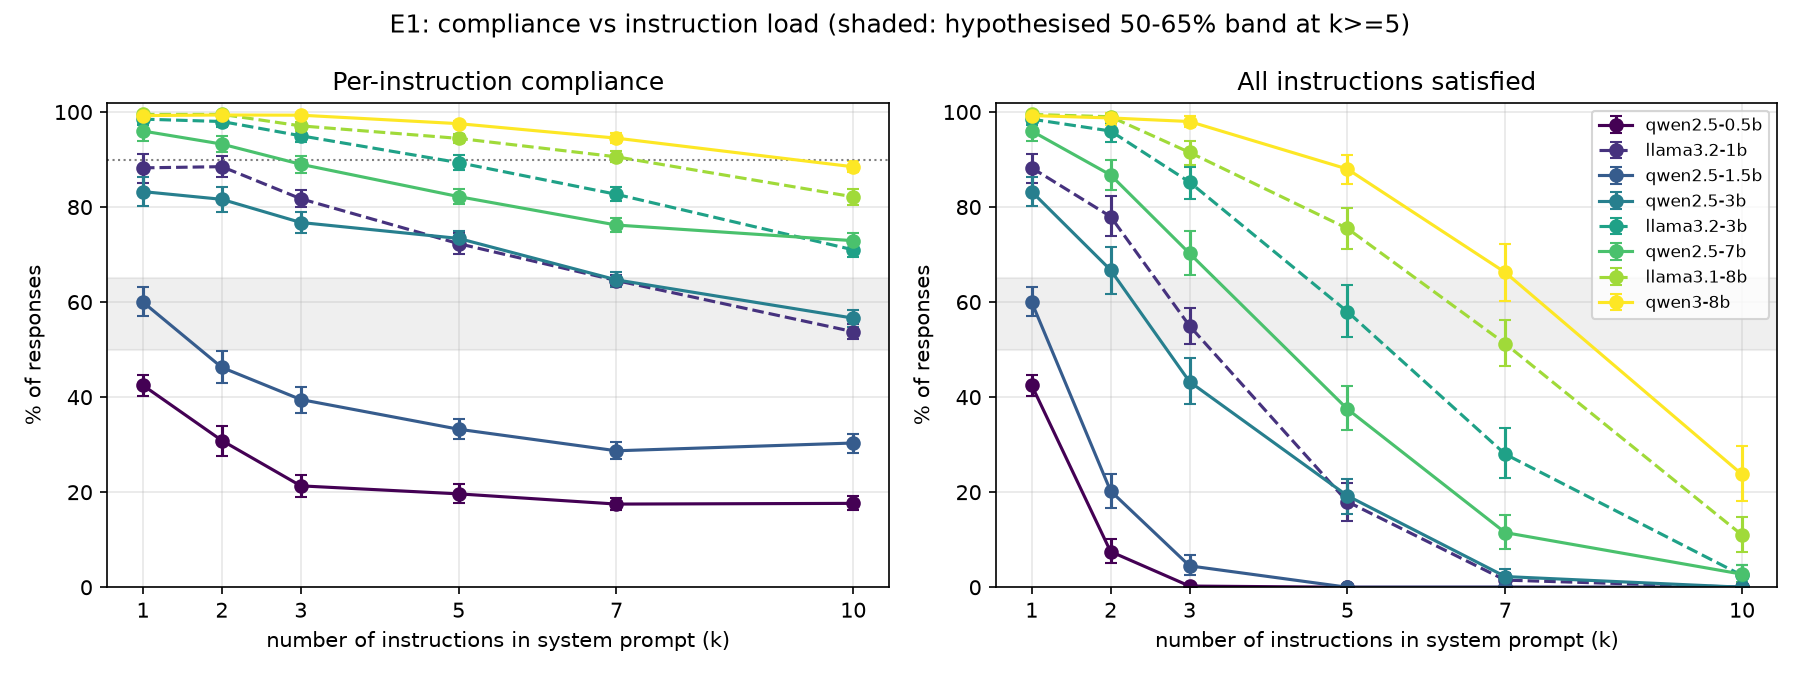
\includegraphics[width=0.95\linewidth]{figures/e1_load_curve.png}
\caption{Compliance against instruction count. \figleft Per-instruction compliance declines roughly linearly for most models, with a floor near 18\% for \qhalf. \figright The all-satisfied rate collapses, and no model exceeds 24\% at $k=10$. Shaded band: the hypothesized 50--65\% range at $k \geq 5$. Error bars: 95\% CIs.}
\label{fig:e1}
\end{figure}

\para{H1 is partially supported.} Single-instruction compliance exceeds 90\% for only 4 of 8 models. The small Qwen2.5 models often fail even one instruction (\qhalf 42.5\%, \qone 60.0\%). With $k \geq 5$, per-instruction compliance ranges from 18\% to 92\% depending on the model. The hypothesized 50--65\% band fits the mid-size models (\lone 61\%, \qthree 63\%) and the $k=10$ cross-model mean, but it does not fit the strongest models (88--92\%) or the weakest (18--30\%).

\para{Load does not hit all instructions equally.} \Tabref{tab:perinstruction} shows that among capable models, \ins{P_name} falls by 47\pp from $k=1$ to $k=10$, while \ins{L_max} falls by 6\pp. \ins{S_nocomma} even rises slightly, from 86.2\% to 90.7\%, because bullets, titles, and word limits shorten answers.

\begin{table}[t]
\centering
\caption{E1: per-instruction compliance (\%), with all-satisfied rate in parentheses. Bootstrap 95\% CI half-widths are about 3\pp or less. Best result per column in \textbf{bold}.}
\label{tab:e1}
\begin{tabular}{@{}lcccccc@{}}
\toprule
\textbf{Model} & $k=1$ & $k=2$ & $k=3$ & $k=5$ & $k=7$ & $k=10$ \\
\midrule
\qhalf & 42.5 & 30.9 (7.5) & 21.3 (0.2) & 19.6 (0.0) & 17.5 (0.0) & 17.6 (0.0) \\
\lone & 88.2 & 88.5 (78.0) & 81.8 (55.0) & 72.3 (18.0) & 64.5 (1.5) & 53.8 (0.0) \\
\qone & 60.0 & 46.2 (20.2) & 39.5 (4.5) & 33.2 (0.0) & 28.7 (0.0) & 30.4 (0.0) \\
\qthree & 83.2 & 81.6 (66.8) & 76.8 (43.2) & 73.4 (19.2) & 64.7 (2.2) & 56.6 (0.0) \\
\lthree & 98.5 & 98.0 (96.0) & 95.0 (85.2) & 89.4 (58.0) & 82.7 (28.0) & 71.0 (2.5) \\
\qseven & 96.0 & 93.2 (86.8) & 89.0 (70.2) & 82.2 (37.5) & 76.2 (11.5) & 72.9 (2.8) \\
\leight & \textbf{99.5} & \textbf{99.5} (\textbf{99.0}) & 97.1 (91.5) & 94.4 (75.5) & 90.6 (51.2) & 82.2 (11.0) \\
\qeight & 99.2 & 99.4 (98.8) & \textbf{99.3} (\textbf{98.0}) & \textbf{97.6} (\textbf{88.0}) & \textbf{94.5} (\textbf{66.2}) & \textbf{88.5} (\textbf{23.8}) \\
\midrule
Mean & 83.4 & 79.7 (69.1) & 75.0 (56.0) & 70.3 (37.0) & 64.9 (20.1) & 59.1 (5.0) \\
\bottomrule
\end{tabular}
\end{table}

\begin{table}[t]
\centering
\caption{E1 compliance (\%) by instruction, averaged over the six capable models. Name and bullet compliance fall steeply, while the word limit and no-comma rules barely move.}
\label{tab:perinstruction}
\resizebox{\textwidth}{!}{%
\begin{tabular}{@{}lcccccccccc@{}}
\toprule
& \ins{F_title} & \ins{F_bullets} & \ins{F_end} & \ins{L_max} & \ins{P_ahoy} & \ins{P_name} & \ins{P_matey} & \ins{S_lower} & \ins{S_nocomma} & \ins{S_keyword} \\
\midrule
$k=1$ & 97.5 & 95.0 & 91.2 & 99.6 & 100.0 & 93.3 & 100.0 & 89.2 & 86.2 & 89.2 \\
$k=5$ & 83.8 & 82.3 & 74.8 & 95.6 & 83.5 & 79.0 & 92.0 & 84.6 & 93.4 & 80.7 \\
$k=10$ & 67.7 & 57.9 & 57.5 & 93.7 & 70.2 & 45.9 & 90.5 & 68.1 & 90.7 & 66.1 \\
\bottomrule
\end{tabular}}
\end{table}


\subsection{Pairwise interference (E2, H2)}

\para{{\bf Do format and length rules suppress persona and style rules?}} \Tabref{tab:e2} shows that the direction holds for some models, but the hypothesized size does not hold in general. Persona and style instructions lose more next to a format or length partner than next to a persona or style partner in 4 of 8 models, with an extra drop of 5--12\pp. Drops of about 20\pp appear only in the two smallest Qwen models, and in those models persona and style partners also cause drops (\qhalf $-$16.9\pp). \lthree, \leight, and \qeight show no effect.

\begin{table}[t]
\centering
\caption{E2: change in persona/style (P/S) compliance relative to the same instruction alone, by partner group (pp). * marks Holm-adjusted $p<.05$. The contrast is the extra drop from a format/length (F/L) partner; \textbf{bold} contrasts have a 95\% CI that excludes 0.}
\label{tab:e2}
\begin{tabular}{@{}lccc@{}}
\toprule
\textbf{Model} & \textbf{F/L partner} & \textbf{P/S partner} & \textbf{Contrast (F/L $-$ P/S) [95\% CI]} \\
\midrule
\qhalf & $-$21.6* & $-$16.9* & \textbf{$-$4.7} [$-$9.1, $-$0.5] \\
\lone & $-$5.7 & +2.1 & \textbf{$-$7.8} [$-$11.4, $-$4.1] \\
\qone & $-$19.5* & $-$7.3 & \textbf{$-$12.2} [$-$17.6, $-$7.2] \\
\qthree & $-$3.4 & $-$0.8 & $-$2.6 [$-$7.6, 2.9] \\
\lthree & $-$0.3 & +0.2 & $-$0.5 [$-$2.4, 1.4] \\
\qseven & $-$6.2 & $-$1.5 & \textbf{$-$4.8} [$-$8.3, $-$1.1] \\
\leight & +1.0 & +0.4 & +0.6 [$-$0.5, 2.1] \\
\qeight & 0.0 & +0.8 & $-$0.8 [$-$2.0, 0.2] \\
\bottomrule
\end{tabular}
\end{table}


\para{Interference is specific, not categorical.} \Figref{fig:e2} shows the full matrix for the six models with single-instruction compliance of at least 80\%. Large cells include \partnerarrow{F_bullets}{F_end} ($-$30\pp), \partnerarrow{F_bullets}{S_keyword} ($-$20\pp), \partnerarrow{S_nocomma}{F_end} ($-$15\pp), \partnerarrow{F_bullets}{P_name}, \partnerarrow{L_max}{S_keyword}, and \partnerarrow{P_matey}{P_name} (each $-$12\pp), and \partnerarrow{P_ahoy}{P_name} ($-$11\pp). The strongest effect is format on format, which H2 does not anticipate. \qthree shows it most clearly: format and length targets with a format or length partner drop 19\pp (Holm-adjusted $p<.001$). The \partnerarrow{F_title}{P_ahoy} cell, which appears as $-$12\pp in \figref{fig:e2}, is mostly a verifier artifact (\secref{sec:sensitivity}).

\begin{figure}[t]
\centering
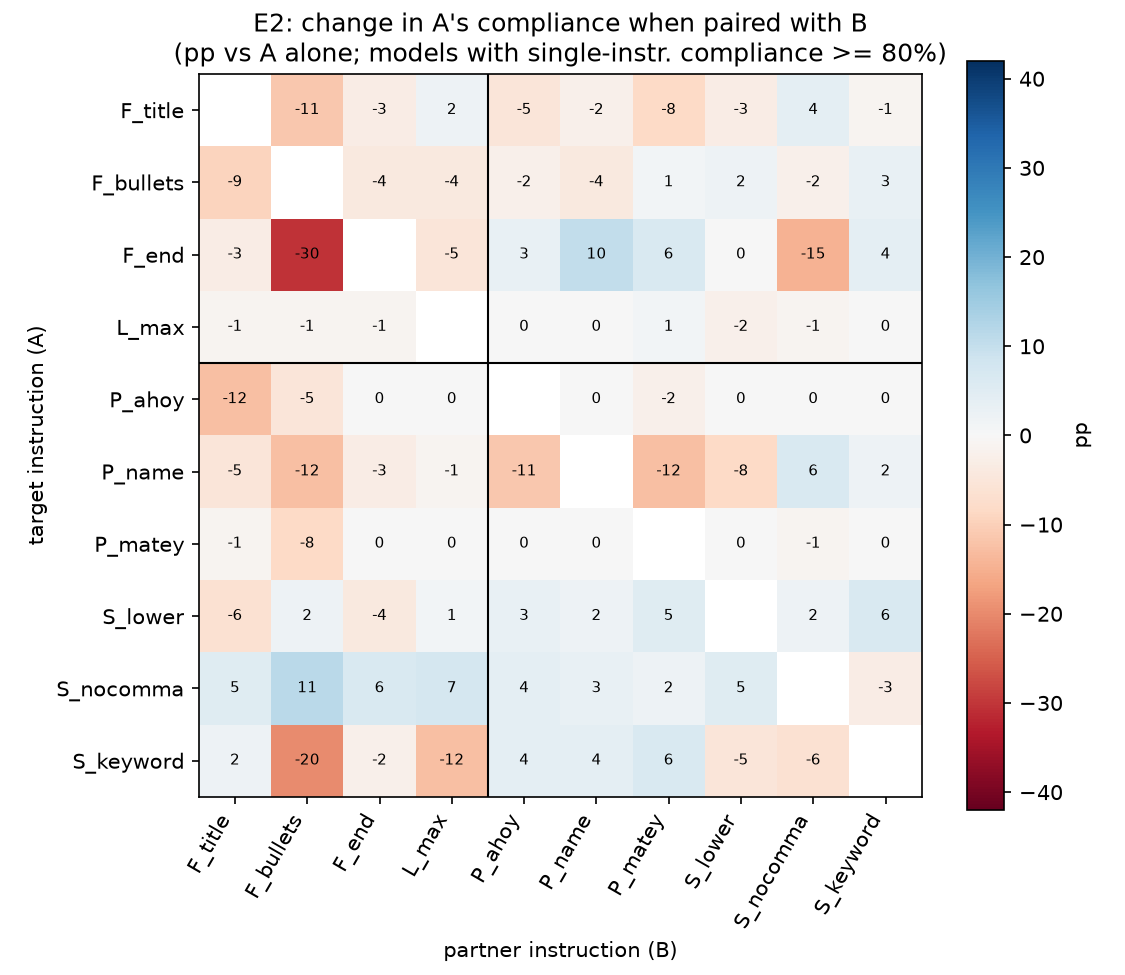
\includegraphics[width=0.62\linewidth]{figures/e2_interference_matrix_capable.png}
\caption{Change in target A's compliance when paired with partner B, relative to A alone on the same task (pp), averaged over the six capable models. Each model contributes 16 responses per cell. Large drops sit in a few cells, mainly the \ins{F_bullets} column. The \ins{S_nocomma} row shows facilitation. The \ins{F_title}/\ins{P_ahoy} cell is inflated by the verifier issue in \secref{sec:sensitivity}.}
\label{fig:e2}
\end{figure}

\para{Large cells vary by model.} These means hide strong differences. \partnerarrow{F_bullets}{F_end} ranges from $-$69\pp for \lthree to 0\pp for \qeight. \partnerarrow{S_nocomma}{F_end} comes entirely from two Llama models (\lthree $-$69\pp, \lone $-$19\pp), and the other four models show 0\pp. \partnerarrow{P_ahoy}{P_name} comes mainly from \qthree ($-$56\pp). With 16 responses per model and cell, these per-model values are noisy.

\para{{\bf Why do these pairs interfere?}} Failure inspection points to \emph{layout capture}. With ``exactly 3 bullets'', models tend to output only the bullets and drop whatever must live outside them. In the \partnerarrow{F_bullets}{F_end} cell, none of the 40 failures among the 96 capable-model responses contains the closing phrase at all. Similarly, a response that opens with ``Ahoy! Ahoy there, matey!'' satisfies the opening but can crowd out the self-introduction.

\para{Some pairs help.} \ins{S_nocomma} gains 5--11\pp next to \ins{F_title}, \ins{F_bullets}, \ins{F_end}, and \ins{L_max}, because structured or shorter answers contain fewer commas.

\subsection{Position (E3, H3)}

\para{{\bf Does the last instruction win?}} H3 is not supported in magnitude. \Tabref{tab:e3} shows a small overall recency advantage of +1.7\pp [0.8, 2.7], and no model reaches the hypothesized +15\pp. Only two models show a Holm-significant effect: \qthree (+8.2\pp) and \qeight (+5.2\pp, failures fall from 7\% to 2\%). Llama models show no recency benefit. The random orders in E1 agree: last-third minus first-third compliance is +5.5\pp for \qeight and +4.9\pp for \qthree, and it ranges from $-$3.1\pp to +1.3\pp for Llama models.

\begin{table}[t]
\centering
\caption{E3: target compliance (\%) by position among 5 instructions. $p$ values are Holm-adjusted across models; the pooled row is unadjusted. \textbf{Bold} marks $p<.05$.}
\label{tab:e3}
\begin{tabular}{@{}lcccc@{}}
\toprule
\textbf{Model} & \textbf{First} & \textbf{Last} & \textbf{Last $-$ first [95\% CI]} & $p$ \\
\midrule
\qhalf & 20.2 & 23.2 & +3.0 [0.7, 5.5] & .20 \\
\lone & 77.0 & 73.2 & $-$3.8 [$-$8.0, 0.8] & .50 \\
\qone & 34.0 & 32.0 & $-$2.0 [$-$6.2, 2.0] & 1.0 \\
\qthree & 65.8 & 74.0 & \textbf{+8.2} [4.2, 12.5] & .005 \\
\lthree & 89.2 & 88.0 & $-$1.2 [$-$4.2, 2.0] & 1.0 \\
\qseven & 80.8 & 84.0 & +3.2 [0.0, 6.5] & .45 \\
\leight & 94.5 & 95.0 & +0.5 [$-$1.2, 2.2] & 1.0 \\
\qeight & 93.0 & 98.2 & \textbf{+5.2} [3.0, 7.5] & $<$.001 \\
\midrule
All models & 69.3 & 71.0 & \textbf{+1.7} [0.8, 2.7] & .002 \\
\bottomrule
\end{tabular}
\end{table}


\subsection{Repetition (E4, H4)}

\para{{\bf Is repetition a free improvement?}} H4 holds in direction but not in magnitude. \Tabref{tab:e4} shows that repeating an instruction raises its compliance by +3.3\pp. The largest gains are in \qone (+6.8\pp) and \qseven (+6.0\pp), and no model reaches +10\pp. The other instructions lose 0.9\pp, far below the hypothesized 5--8\pp. A neutral filler line in the same slot causes the same loss, and repeat and filler do not differ for the other instructions (+0.1\pp [$-$0.5, 0.6]). So the collateral cost comes from a longer prompt, not from repetition. \Figref{fig:e3e4} shows per-model results.

\begin{table}[t]
\centering
\caption{E4: repetition effects in pp [95\% CI], pooled over 8 models (3,200 paired items per condition).}
\label{tab:e4}
\begin{tabular}{@{}lccc@{}}
\toprule
\textbf{Measure} & \textbf{Repeat $-$ base} & \textbf{Repeat $-$ filler} & \textbf{Filler $-$ base} \\
\midrule
Repeated instruction & \textbf{+3.3} [2.2, 4.5] & \textbf{+4.4} [3.2, 5.5] & $-$1.0 [$-$2.1, 0.0] \\
Other 4 instructions & \textbf{$-$0.9} [$-$1.4, $-$0.3] & +0.1 [$-$0.5, 0.6] & \textbf{$-$0.9} [$-$1.4, $-$0.5] \\
\bottomrule
\end{tabular}
\end{table}


\begin{figure}[t]
\centering
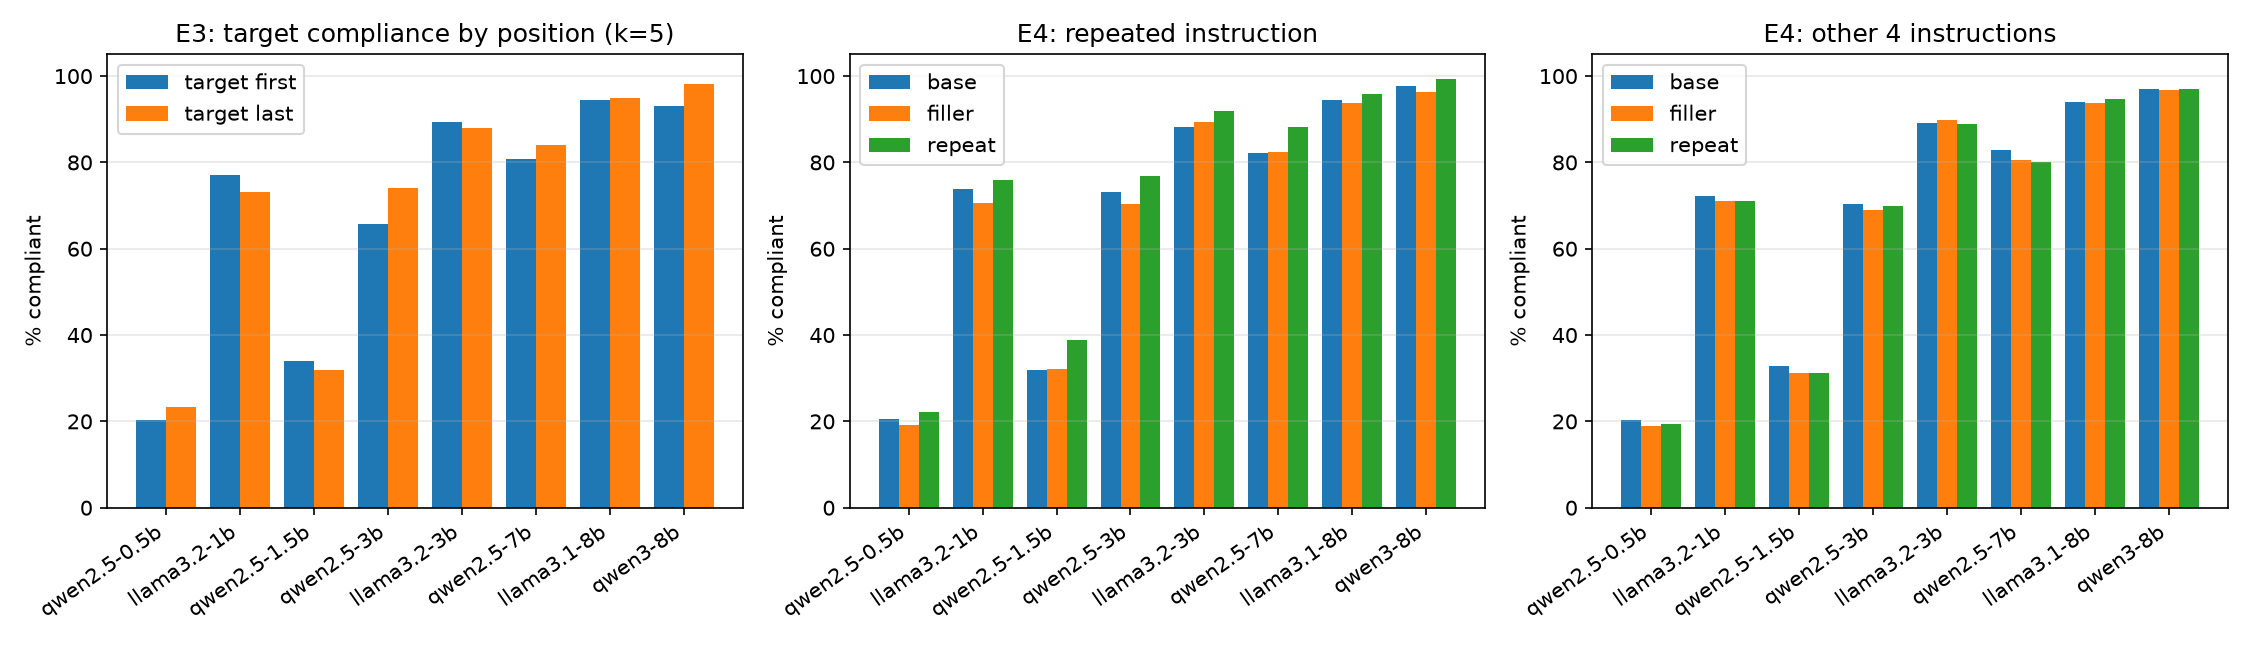
\includegraphics[width=0.95\linewidth]{figures/e3_e4_position_repetition.png}
\caption{\figleft E3: target compliance when placed first or last. \figcenter E4: compliance of the repeated instruction under base, filler, and repeat conditions. \figright E4: compliance of the other 4 instructions. Differences between conditions are small compared with differences between models.}
\label{fig:e3e4}
\end{figure}

\subsection{Model size (H5)}

\para{{\bf Do smaller models decay faster?}} The answer depends on the scale (\tabref{tab:h5}). Relative to their own baseline, smaller models lose much more: \qhalf loses 57\% of its compliance, while \qeight loses 7\% (Spearman $\rho=-0.95$, $p<.001$). In absolute pp per added instruction there is no size trend ($\rho=0.07$, $p=.87$), because floor models have little left to lose and ceiling models lose slowly at first. On the logit scale, the trend points the other way, but it is not significant across 8 models ($\rho=-0.64$, $p=.09$): \qeight multiplies its odds by 0.65 per added instruction, and \qhalf by 0.83. Family matters too, since Llama models have steeper logit slopes than Qwen2.5 models of similar size.

\begin{table}[t]
\centering
\caption{H5: decay by model size. The slope is pp per added instruction, the relative drop compares $k=1$ with $k \geq 5$, and the logit slope comes from the logistic GLM (95\% CIs in brackets). Models are sorted by size. Shallowest slope and smallest drop in \textbf{bold}.}
\label{tab:h5}
\resizebox{\textwidth}{!}{%
\begin{tabular}{@{}lcccc@{}}
\toprule
\textbf{Model} & \textbf{Params (B)} & \textbf{Slope (pp)} & \textbf{Relative drop} & \textbf{Logit slope} \\
\midrule
\qhalf & 0.5 & \textbf{$-$1.30} [$-$1.48, $-$1.14] & 57\% & $-$0.18 [$-$0.21, $-$0.16] \\
\lone & 1.2 & $-$3.99 [$-$4.21, $-$3.75] & 30\% & $-$0.24 [$-$0.26, $-$0.23] \\
\qone & 1.5 & $-$1.80 [$-$2.15, $-$1.46] & 49\% & \textbf{$-$0.13} [$-$0.16, $-$0.11] \\
\qthree & 3.1 & $-$3.05 [$-$3.35, $-$2.76] & 24\% & $-$0.18 [$-$0.20, $-$0.16] \\
\lthree & 3.2 & $-$3.36 [$-$3.56, $-$3.14] & 20\% & $-$0.35 [$-$0.37, $-$0.33] \\
\qseven & 7.6 & $-$2.38 [$-$2.62, $-$2.12] & 21\% & $-$0.20 [$-$0.23, $-$0.18] \\
\leight & 8.0 & $-$2.15 [$-$2.40, $-$1.89] & 12\% & $-$0.34 [$-$0.38, $-$0.30] \\
\qeight & 8.2 & $-$1.47 [$-$1.63, $-$1.30] & \textbf{7\%} & $-$0.44 [$-$0.49, $-$0.39] \\
\bottomrule
\end{tabular}}
\end{table}


\subsection{Robustness: numbered lists}

We rerun E1 and E3 with numbered instructions on four models. Load curves barely change. Compliance at $k=1/5/10$ moves from 98.5/89.4/71.0 to 98.5/89.0/71.1 for \lthree, from 83.2/73.4/56.6 to 86.2/70.3/53.4 for \qthree, and from 99.2/97.6/88.5 to 99.8/98.0/92.6 for \qeight. Numbering helps \qeight by 4\pp at $k=10$ and hurts \qthree by 3\pp. Position signs are unchanged: \qthree +7.0\pp, \qeight +3.0\pp, \lthree $-$3.0\pp, and \qone $-$3.8\pp.

\subsection{Verifier sensitivity}
\label{sec:sensitivity}

\Tabref{tab:sensitivity} reports the full analysis rerun with the corrected \ins{P_ahoy} check from \secref{sec:method}. Our main conclusions hold: count stays dominant, position and repetition stay small, and the Spearman results for H5 are unchanged to the reported precision. The same four models keep a contrast that excludes 0 in \tabref{tab:e2}. Two details change. First, the \partnerarrow{F_title}{P_ahoy} interference is mostly an artifact: it shrinks from $-$12.5\pp to $-$3.1\pp, and \qthree rises from 50\% to 100\% in this cell, so we do not count it as evidence of layout capture. Second, the \qthree recency effect shrinks to +6.5\pp, although it stays significant.

\begin{table}[t]
\centering
\caption{Effect of the corrected \ins{P_ahoy} verifier on the results that change most. Other pooled results move by less than 1\pp. Across E1, the largest single-model shifts are 1.7\pp in compliance and 4.3\pp in the all-satisfied rate, both at $k=5$ and in the models listed here.}
\label{tab:sensitivity}
\begin{tabular}{@{}llcc@{}}
\toprule
\textbf{Experiment} & \textbf{Result} & \textbf{Original} & \textbf{Corrected} \\
\midrule
E1 & Mean compliance, $k=5$ / $k=10$ & 70.3 / 59.1 & 70.7 / 59.3 \\
E1 & Mean all-satisfied rate, $k=5$ / $k=10$ & 37.0 / 5.0 & 38.2 / 5.0 \\
E1 & \qthree all-satisfied rate, $k=5$ & 19.2 & 23.5 \\
E1 & \lone all-satisfied rate, $k=5$ & 18.0 & 22.2 \\
E2 & \partnerarrow{F_title}{P_ahoy}, capable models (pp) & $-$12.5 & $-$3.1 \\
E2 & \qthree F/L $-$ P/S contrast (pp) & $-$2.6 & $-$0.5 \\
E3 & All models, last $-$ first (pp) & +1.7 ($p=.002$) & +1.4 ($p=.009$) \\
E3 & \qthree, last $-$ first (pp) & +8.2 ($p=.005$) & +6.5 ($p=.035$) \\
E4 & Repeated instruction, repeat $-$ base (pp) & +3.3 & +3.5 \\
E4 & Repeated instruction, filler $-$ base (pp) & $-$1.0 & $-$0.8 \\
\bottomrule
\end{tabular}
\end{table}


\section{Discussion}
\label{sec:discussion}

\para{Count dominates, and it compounds.} Per-instruction compliance falls by about 1.5--4\pp per added instruction across capable models, so the chance of meeting every constraint collapses. This matches the multi-constraint literature \citep{harada2025multiply}, and we show it here in a controlled system-prompt setting. For practitioners, a 10-rule system prompt is fully obeyed in at most 24\% of responses, even by the best model we test. If every rule must hold, shorten the prompt or check outputs with code.

\para{Interference is local.} H2 framed interference as format against persona. Our data point to layout capture instead: an instruction that fixes the overall shape of the response displaces content that must live outside that shape. Some combinations also help each other. Because large cells vary so much by model, a small pairwise test on the target model before deployment is more informative than a general rule. Layout capture is our reading of inspected failures, not a tested causal claim, and an explicit output template would be a natural test of it.

\para{Ordering and repetition are weak levers.} Recency effects exist in some Qwen models, but they amount to a few pp and do not appear in Llama models. Repetition gains about 3\pp on average, and its cost to other instructions is simply the cost of a longer prompt.

\para{Size helps compliance, not robustness to load.} Larger models start near the ceiling and stay higher in absolute terms. However, we do not find that they lose odds of compliance more slowly per added instruction. The claim that smaller models decay faster holds only relative to each model's own baseline, and that scale favors high-baseline models.

\para{Limitations.} We test only open models up to 8B, so frontier models may need $k>10$ to show the same regime, and most local models are 4-bit quantized. Our 10 instructions are lexical proxies: persona checks test markers such as ``Ahoy'', not overall voice. Each category has only 3--4 instructions, so category effects are confounded with the choice of instructions, and H2 claims are weak at the category level. The pool also does not test instructions that conflict. We use greedy decoding with one run per prompt, so variance comes from tasks and instruction subsets, not sampling. Earlier work on this host found that vLLM greedy outputs can change slightly with batch composition, so single-model effects of a few pp need caution. Part of the \qseven run was lost and regenerated with the same prompts and settings but different batching. Pairwise cells have few responses per model. We found the \ins{P_ahoy} verifier issue after the main analysis, and we corrected it only in a post-hoc sensitivity analysis. Finally, our related work rests on background knowledge because no literature search stage ran.

\section{Conclusion}
\label{sec:conclusion}

We run a controlled study of verifiable instructions in system prompts across 8 open-weight models. Instruction count is the main driver of non-compliance: per-instruction compliance falls by about 1.5--4\pp per added instruction for capable models, and the all-satisfied rate falls to 37.0\% at five instructions and 5.0\% at ten. Placing an instruction last (+1.7\pp) and repeating it (+3.3\pp) help only a little, and repetition has no cost beyond prompt length. Interference concentrates in specific pairs, especially instructions that fix the whole response layout, rather than in broad format-versus-persona competition. Smaller models do worse at every load, but they are not clearly less robust to added load once floor and ceiling effects are considered.

The key takeaway is simple: to improve compliance, remove instructions rather than rearrange them.

Next, we plan to test frontier models with $k$ up to 20--30, use judged persona and tone instructions, test output templates as a mitigation for layout capture, sample at $T>0$ with multiple seeds to separate decoding noise from small effects, and test whether pairwise interference in E2 predicts failures at higher $k$.


\bibliography{references}
\end{document}
